\documentclass[12pt,openright,oneside,a4paper,english,french,spanish,table,xcdraw]{abntex2}

% Pacotes
\usepackage{cmap}	
\usepackage{lmodern}	
\usepackage[T1]{fontenc}	
\usepackage[utf8]{inputenc}		
\usepackage{lastpage}		
\usepackage{indentfirst}
\usepackage{color, colortbl}
\usepackage{graphicx}	
\usepackage{units}
\usepackage[brazilian,hyperpageref]{backref}
\usepackage{bold-extra}
\usepackage{eso-pic}
\usepackage{tabularx}
\usepackage[alf]{abntex2cite}
\usepackage{pgfgantt}
\usepackage{pdflscape}
\usepackage{mdframed}
\usepackage{minted}
\usepackage{dirtree}
\usepackage{float}
\usepackage{adjustbox}
\usepackage{fontawesome5}
\usepackage{booktabs}
\usepackage{geometry}
\usepackage{hyperref}
\usepackage{amsfonts}
\usepackage{caption}
\usepackage{subcaption}
\usepackage{tikz}
\usetikzlibrary{shapes.geometric, arrows.meta, positioning, decorations.pathreplacing}
\usepackage{booktabs} % Para linhas de tabela mais profissionais
\usepackage{tabularx} % Para tabelas com colunas de largura ajustável
\usepackage{multirow} % Para células que ocupam múltiplas linhas
\usepackage{pgfgantt}
\usepackage{ragged2e}
\geometry{a4paper, margin=1in}

\usepackage{fixos/customizacoes}

% Custom colors
\definecolor{LightBlue}{rgb}{0.67,0.82,1}
\definecolor{Gray}{gray}{0.9}
\definecolor{White}{rgb}{1,1,1}
\definecolor{UnB_Azul}{HTML}{003366}
\definecolor{UnB_Verde}{HTML}{006633}

\renewcommand{\backrefpagesname}{Citado na(s) página(s):~}
\renewcommand{\backref}{}
\renewcommand*{\backrefalt}[4]{
	\ifcase #1 %
		Nenhuma citação no texto.%
	\or
		Citado na página #2.%
	\else
		Citado #1 vezes nas páginas #2.%
	\fi}%
% ---

\makeatletter
\AtBeginDocument{%
  \newcommand\My@Macro[1]{#1}%
  \newcommand\My@Thirdoffive[5]{\My@Macro{#3}}%
  \renewcommand*\@namerefstar[1]{%
    \HyRef@StarSetRef{#1}\My@Thirdoffive
  }%
  \renewcommand*\T@nameref[1]{%
    \begingroup
    \let\label\@gobble
    \NR@setref{#1}\My@Thirdoffive{#1}%
    \endgroup
  }%
  \DeclareRobustCommand\fucnameref{%
    \@ifstar\fucnameref@star\fucnameref@nostar
  }%
  \newcommand\callemakefirstuc[1]{%
    \MakeLowercase{\emakefirstuc{#1}}%
  }%
  \newcommand\fucnameref@star[1]{%
    \begingroup
    \let\My@Macro=\callemakefirstuc
    \nameref*{#1}%
    \endgroup
  }%
  \newcommand\fucnameref@nostar[1]{%
    \begingroup
    \let\My@Macro=\callemakefirstuc
    \nameref{#1}%
    \endgroup
  }%
  \DeclareRobustCommand\ucnameref{%
    \@ifstar\ucnameref@star\ucnameref@nostar
  }%
  \newcommand\ucnameref@star[1]{%
    \begingroup
    \MFUhyphentrue
    \let\My@Macro=\ecapitalisefmtwords
    \nameref*{#1}%
    \endgroup
  }%
  \newcommand\ucnameref@nostar[1]{%
    \begingroup
    \MFUhyphentrue
    \let\My@Macro=\ecapitalisefmtwords
    \nameref{#1}%
    \endgroup
  }%
  \DeclareRobustCommand\lcnameref{%
    \@ifstar\lcnameref@star\lcnameref@nostar
  }%
  \newcommand\lcnameref@star[1]{%
    \begingroup
    \let\My@Macro=\MakeLowercase
    \nameref*{#1}%
    \endgroup
  }%
  \newcommand\lcnameref@nostar[1]{%
    \begingroup
    \let\My@Macro=\MakeLowercase
    \nameref{#1}%
    \endgroup
  }%
}%
\makeatother
% Dados pessoais
\autor{Matheus Pimentel Leal}
\curso{Engenharia de Software}

% Dados do trabalho
\titulo{Math Hero: Um Jogo Educacional para o Ensino de Matemática}
\data{2025}
\palavraChaveUm{Engenharia de Games}
\palavraChaveDois{Engenharia de Software}

% Dados da orientacao
\orientador{Dr. Edson Alves da Costa Júnior}
%coorientador{quando houver, Titulação Acadêmica e Nome do Orientador}

% Dados para a ficha catalográfica
\cdu{02:141:005.6}

% Dados da aprovação do trabalho
\dataDaAprovacao{14 de Fevereiro de 2025}
\membroConvidadoUm{Dr.ª Carla Silva Rocha Aguiar}
\membroConvidadoDois{Dr. Matheus Bernardini de Souza}

% Dados pessoais
\autor{Matheus Pimentel Leal}
\curso{Engenharia de Software}

% Dados do trabalho
\titulo{Math Hero: Um Jogo Educacional para o Ensino de Matemática}
\data{2025}
\palavraChaveUm{Engenharia de Games}
\palavraChaveDois{Engenharia de Software}

% Dados da orientacao
\orientador{Dr. Edson Alves da Costa Júnior}
%coorientador{quando houver, Titulação Acadêmica e Nome do Orientador}

% Dados para a ficha catalográfica
\cdu{02:141:005.6}

% Dados da aprovação do trabalho
\dataDaAprovacao{14 de Fevereiro de 2025}
\membroConvidadoUm{Dr.ª Carla Silva Rocha Aguiar}
\membroConvidadoDois{Dr. Matheus Bernardini de Souza}

\input{fixos/setup}

\begin{document}

    \frenchspacing 
    \imprimircapa
    \imprimirfolhaderosto

    \input{fixos/fichaCatalografica.tex}
    %\input{editaveis/errata.tex}
    \input{fixos/folhaDeAprovacao.tex}
    % \begin{dedicatoria}
   \vspace*{\fill}
   \centering
   \noindent

   \textit{Este trabalho é dedicado às crianças adultas que,\\
   quando pequenas, se apaixonaram por games.
   } \vspace*{\fill}
\end{dedicatoria}

    % \begin{agradecimentos}
Agradeço primeiramente a Deus, que me abençoou com a oportunidade de realizar este projeto que pode vir a causar grande impacto na vida de jovens e adolescentes, e também aos que estão apenas buscando novas maneiras de aprendizado. Por ter me abençoado com essa vida, por ter colocado tantas pessoas incríveis ao meu redor, por me dar saúde, por me proporcionar a oportunidade de servir por meio do meu trabalho e do meu conhecimento.

Agradeço imensamente a meus pais, Walderico de Fontes Leal e Alda Dias Pimentel Leal, pelo apoio incondicional, pelo amor, pela paciência, pelas horas dedicadas à minha educação, por terem me proporcionado uma infância cheia de amor, feliz e rica em amizades. Sem o apoio de vocês nada do que conquistei e nada do que sou seria possível. Obrigado Pai, por sempre acreditar no meu potencial, por me ensinar a ser um homem íntegro e ter bom coração. Obrigado mãe, por me ensinar a delicadeza, por ser minha maior incentivadora, por todo sacrifício feito, por todas as noites que a senhora passou em claro para cuidar de mim e por me mostrar que a resiliência e a paciência vencem qualquer obstáculo.

Agradeço ao meu irmão, Samuel Pimentel Leal, pelos anos de cuidado, companheirismo, carinho e amor. Obrigado por me ensinar que as diferenças entre as pessoas são o que as tornam únicas. Obrigado por me acompanhar e me proteger na minha inocência quando criança, por ter sido referência na busca por conhecimento, por me mostrar que sou mais capaz e corajoso do que imagino.

Agradeço à minha segunda mãe, Maria da Conceição da Silva, por ser inspiração de superação, de força, de coragem e de dedicação à Cristo. Por me mostrar que mesmo com grandes adversidades em nossas vidas ainda temos motivos para sorrir e acreditar. Por sempre cuidar de mim, por me amar mesmo não sendo teu filho de sangue e por me dar o enorme prazer de dizer à todos que encontro que tenho duas mães.

Agradeço à minha avó e madrinha, Maria Conceição Gomes Pimentel e minha tia Denise Dias Pimentel, por serem pilares de uma família amorosa e cheia de pessoas que procuram sempre fazer o bem. Obrigado por todos os momentos de amor compartilhados, por toda paciência comigo e por me terem me ensinado que o cuidado e o carinho para com os que amamos é incondicional.

Agradeço à minha noiva e futura esposa, Giulia Lobo Barros, com quem partilho a vida há 4 anos. Por ser minha parceira em todos os momentos, por me dar amor e carinho todos os dias, especialmente nos que não estou bem. Por me reintroduzir à minha espiritualidade, por ser minha companheira na vida espiritual. Obrigado por me ajudar a carregar meus fardos, por me inspirar a ser melhor e por me mostrar que o dom do perdão é libertador.

Agradeço ao meu padrinho, José Carlos Leal, por cuidar de mim, me aconselhar, por ser presente na minha vida e por ser uma das maiores inspirações de paciência que tenho na vida.

Agradeço à toda a família da minha noiva por ter me recebido de braços abertos, pelos conselhos, pela ajuda, pelo carinho e por me proporcionarem alegria em todos os momentos que estamos juntos.

Agradeço aos irmãos que a vida me deu: Eduardo Souto Reis, Ricardo Cipriano Guimarães Gomes e Felipe Lademir Filippin. Vocês entraram na minha vida e por opção própria permaneceram e assim criamos o vínculo forte que temos hoje. Obrigado por serem meus melhores amigos de vida, pelos conselhos amorosos, pelos conselhos de vida, pela amizade, pelas risadas, por terem me abençoado com a amizade de vocês.

Obrigado à minha amiga, Daniela Ferreira de Oliveira, por ter me mostrado o inúmeros benefícios da psicologia, por não ter desistido de saber se eu estava bem até quando eu te afastei. Obrigado pelas inúmeras risadas, por ter sido luz em um momento de escuridão.

Agradeço ao meu parceiro de organização da \textit{Game Jam FGA}, Liverson Paulo Furtado Severo, que dividiu comigo a organização deste evento que com tanto carinho idealizei. Nossas conversas e ideias me trazem inspiração para correr atrás de meus sonhos. Se não fosse pela ajuda dele, nem este trabalho e nem a \textit{Game Jam FGA} tomariam forma.

Gostaria de agradecer também aos meus companheiros de FCTE: Ícaro Oliveira, Kalliu Brasil, Lude Ribeiro, Pedro Dias, Priscilla Rath e Lucas Régis. Cheguei na FCTE sem pretensão alguma de formar grandes laços de amizade e vocês foram uma surpresa incrível. Um agradecimento especial vai para o Ícaro, por me encher a paciência para trocar para o curso de Engenharia de Software, e, alguns anos depois, cá estou.

Agradeço ao professor Dr. Edson Alves da Costa Júnior, pelas incontáveis horas de parceria firmadas por meio da realização de trabalhos importantíssimos como este a a \textit{Game Jam FGA}. Obrigado pelos incontáveis conselhos, pela imensa paciência, pelo incentivo e pela grande inspiração que o Sr. se tornou em minha vida. Obrigado pela oportunidade de aprender contigo, seja nas aulas, seja por meio de projetos. Espero que eu possa um dia retribuir tudo o que o Sr. me proporcionou por meio do seu trabalho.

Por último, mas não menos importante, agradeço à toda \textit{BsBeast's} por serem meus amigos e companheiros de jogatina, e também pelas risadas de todo dia no Discord.
\end{agradecimentos}

    % \begin{epigrafe}
    \vspace*{\fill}
	\begin{flushright}
		\textit{``
        As grandes histórias nunca terminam realmente, Sr. Frodo.
        \\ Nem sempre quem as conta vê o fim delas, 
         \\ e quando se vai embora, outra pessoa tem de continuar a contá-las.'' \\
		(O Senhor dos Anéis: O Retorno do Rei)}
	\end{flushright}
\end{epigrafe}

    % \begin{resumo}
 A dificuldade de alunos do ensino básico brasileiro na compreensão do currículo base de matemática não é novidade para os professores. Por isso diversos métodos pedagógicos vêm sendo utilizados a fim de melhorar a fixação dos conteúdos ensinados. Os \textit{serious games} surgiram como proposta de metodologia lúdica para aumentar a fixação dos conteúdos por parte dos alunos, porém, o aspecto lúdico, que é responsável por proporcionar o divertimento dos jogadores, muitas vezes é deixado de lado. Este trabalho utiliza os conceitos da engenharia de \textit{games} e da engenharia de software tradicional para a criação do \textit{game} Math Hero, para auxiliar no ensino de técnicas de cálculo mental para alunos do ensino básico brasileiro. Tendo como base os conceitos citados, foi implementada uma versão \textit{alpha} do jogo que contém uma mistura entre duas modalidades de modo de jogo \textit{time attack} programadas para o desenvolvimento final, a modalidade competição e de treino, para que fosse possível a coleta, a análise e a comparação de dados de jogabilidade entre jogadores com e sem instrução prévia, no evento ``Torneio de matemática mental'' ocorrido durante a Semana de Extensão Universitária 2024 da Universidade de Brasília.
 \vspace{\onelineskip}
    
 \noindent
 \textbf{Palavras-chave}: Engenharia de \textit{Games}. Engenharia de Software. \textit{Games}. Cálculo Mental. Matemática.
\end{resumo}

    % \begin{resumo}[Abstract]
 \begin{otherlanguage*}{english}
   The difficulty of Brazilian elementary school students have in understanding the basic math curriculum is not new to teachers. For this reason, various pedagogical methods are being used to improve the retention of the content taught. Serious games emerged as a play based methodology to increase students' retention of the math curriculum, but the fun aspect, which is responsible for providing players' enjoyment is often overlooked by the genre. This paper uses concepts from game software engineering and traditional software engineering to create the game \textit{Math Hero}, to help teach mental math techniques to Brazillian elementary school students. Based on the aforementioned concepts, a alpha version of the game was implemented that contains a mixture of two game modes time attack programmed for the final development, the competition and training mode, so that it would be possible to collect, analyze and compare gameplay data between players with and without previous instruction, using the ``Mental Math Tournament'' event that took place during the University Extension Week 2024 at the University of Brasilia.
   \vspace{\onelineskip}
 
   \noindent 
   \textbf{Key-words}: Game Engineering. Software Engineering. Games. Mental Math. Mathematics.
 \end{otherlanguage*}
\end{resumo}
    % \input{fixos/listasAutomaticas.tex}
    \begin{siglas}
  \item [BNCC] Base Nacional Comum Curricular
  \item [EG] Engenharia de Games
  \item [ER] Engenharia de Requisitos
  \item [ES] Engenharia de Software
  \item [FCTE] Faculdade de Ciências e Tecnologias em Engenharia
  \item [FGA] Faculdade do Gama
  \item [GDD] \textit{Game Design Document}
  \item [GSE] \textit{Game Software Engineering}
  \item [MEC] Minstério da Educação
  \item [NPC] \textit{Non Playable Character}
  \item [OCDE] Organização para a Cooperação e Desenvolvimento Econômico
  \item [SE] \textit{Software Engineering}
  \item [UnB] Universidade de Brasília
\end{siglas}

    % \input{editaveis/simbolos.tex}
    \input{fixos/indiceAutomatico.tex}

    \textual

    \chapter{Introdução}\label{chapter:introducao}

\section{Contexto}

\subsection{A nova realidade}

\begin{citacao}
``A IA generativa é a tecnologia mais transformadora do nosso tempo, possibilitando avanços em criatividade, produtividade e descoberta científica'' \citeonline{huang_2023}.
\end{citacao}

Desde novembro de 2022, o campo da tecnologia testemunha uma transformação significativa com a ascensão da Inteligência Artificial (IA) generativa, impulsionada pelo lançamento em larga escala do ChatGPT pela OpenAI. Essa ferramenta marcou o início de uma nova era no desenvolvimento de software, redefinindo processos e práticas tradicionais.

Nesse contexto de ``\textit{nova realidade}'', emergem desafios associados a cenários antes considerados distópicos ou restritos à ficção científica. A IA tem transformado profundamente o desenvolvimento de software, introduzindo ferramentas que automatizam e aprimoram processos outrora exclusivos de desenvolvedores humanos. Ferramentas como GitHub Copilot, ChatGPT e Claude, baseadas em IA generativa, permitem a geração de código, sugestões em tempo real e execução de tarefas complexas a partir de comandos em linguagem natural, os chamados \textit{prompts}. Esse cenário redefine a interação entre desenvolvedores e sistemas computacionais, inaugurando um ambiente colaborativo entre humanos e máquinas.

\begin{citacao}
``Eu diria que talvez 20\%, 30\% do código que está em nossos repositórios hoje e em alguns de nossos projetos provavelmente foi todo escrito por software'' \citeonline{nadella_2025}\footnote{As datas futuras em referências de notícias e artigos de opinião refletem a natureza prospectiva e de rápida evolução do tema, posicionando a discussão no contexto do ano de defesa desta monografia.}.
\end{citacao}

A adoção cada vez mais acelerada dessas ferramentas por empresas e comunidades de desenvolvedores levanta questões sobre produtividade, qualidade, segurança e o papel do desenvolvedor no processo de produção de código. Relatórios corporativos, como os da Microsoft e do GitHub, indicam que uma proporção significativa de código já é gerada por IA, evidenciando a escala dessa transformação. Contudo, os impactos reais dessas tecnologias — incluindo benefícios, desafios e riscos — ainda carecem de análises sistemáticas baseadas em dados públicos.

\begin{citacao}
``Como em todas as revoluções tecnológicas, espero que haja um impacto significativo nos empregos, mas é muito difícil prever exatamente como será esse impacto'' \citeonline{altman_2023}.
\end{citacao}

Esta pesquisa é motivada pela necessidade de compreender como a IA está moldando o desenvolvimento de software, tanto em termos técnicos quanto nas dinâmicas de trabalho. A disponibilidade crescente, embora limitada, de dados públicos — como relatórios de empresas e repositórios — oferece uma oportunidade de investigar essas mudanças e contribuir para o debate acadêmico e profissional sobre o futuro da programação.

\subsection{Motivação dos autores}

Como estudantes de Engenharia de Software, vivenciamos um momento de ruptura tecnológica que redefine nossa profissão e o ecossistema ao seu redor. A integração acelerada da IA no desenvolvimento de software suscita dúvidas, expectativas e receios que nos motivam a investigar como tais ferramentas estão transformando os processos de produção de código e o papel dos desenvolvedores.

\begin{citacao}
``Nos próximos 18 meses, a maior parte da codificação será feita por IA, e ela será melhor que o trabalho da maioria dos engenheiros plenos'' \citeonline{zuckerberg_2025}.
\end{citacao}

Declarações como essa, feitas por figuras públicas com grande influência no setor tecnológico, intensificam questionamentos sobre o futuro do trabalho em programação. De modo semelhante, Elon Musk apresenta uma visão ainda mais radical:

\begin{citacao}
``Provavelmente, nenhum de nós terá um emprego [...] Haverá um ponto em que nenhum trabalho será necessário. Você poderá ter um trabalho se quiser ter um trabalho por satisfação pessoal, mas a IA e os robôs fornecerão todos os bens e serviços que você desejar'' \citeonline[tradução nossa]{musk_2024_vivatech}.
\end{citacao}

Embora inseridas em um discurso de ``abundância universal'', tais afirmações funcionam como catalisadores de incertezas, especialmente para estudantes e profissionais em formação.

Além dessas projeções, notícias recentes abordam as dificuldades enfrentadas por profissionais de software no uso de ferramentas de IA, desde iniciantes até desenvolvedores experientes \citeonline{g1_2024}. As percepções sobre o futuro variam entre visões pessimistas e otimistas. Entre os pontos positivistas está a possível diminuição da necessidade do trabalho sistemático de escrita de código.

Segundo Bianchin (2025), Jensen Huang argumenta que não é mais necessário aprender a programar, pois a IA já pode assumir essa função. Nessa perspectiva, engenheiros de software poderiam dedicar mais tempo a atividades que exigem criatividade e inovação \citeonline{xataka_2025}.

Contribuindo com essa visão, McFarland discute o conceito de \textit{Vibe Coding}, no qual modelos de linguagem permitem que qualquer pessoa crie aplicações ao simplesmente descrever ideias em linguagem natural. Ferramentas como Cursor e Lovable integram agentes inteligentes que ampliam o público capaz de desenvolver software \citeonline{mcfarland2025vibe}.

Entretanto, há também visões críticas. Bianchin evidencia preocupações de programadores experientes com a crescente dependência das ferramentas de IA. Para Namanyay Goel, desenvolvedores iniciantes produzem mais código, porém compreendem menos os fundamentos de suas soluções — o que pode gerar consequências futuras \citeonline{xataka_2025}.

Esse cenário demanda mais do que adoção tecnológica: exige transformação estratégica e cultural. Como ressalta \citeonline{salvador_2024}, o uso da IA deve integrar-se cedo ao fluxo de trabalho, sob metas claras, governança robusta de dados, capacitação contínua e estratégias iterativas de implementação.

Questões jurídicas também emergem. Conforme Basilio \cite{basilio_2025}, especialistas divergem sobre a responsabilidade por danos causados por agentes de IA. Empresas podem ser responsabilizadas mesmo quando o erro não se origina nelas, enquanto representantes das desenvolvedoras argumentam que usuários devem assumir parte da responsabilidade ao serem informados sobre limitações dos sistemas. Problemas como ``superengenharia'' — a criação de arquiteturas excessivamente complexas com múltiplos agentes — também são apontados como riscos \cite{basilio_2025}.

Esse conjunto de incertezas motiva a pergunta central deste trabalho:

\begin{citacao}
\textit{Quais são os reais impactos da Inteligência Artificial na produção de código e como eles afetam o futuro do desenvolvimento de software?}
\end{citacao}

Com isso, propomos uma análise crítica dos efeitos da IA, investigando suas aplicações e implicações para produtividade, qualidade e relações de trabalho.

\section{Problema}\label{section:problema}

A rápida adoção de ferramentas de IA no desenvolvimento de software não tem sido acompanhada, de maneira suficiente, por estudos sistemáticos que avaliem seus impactos reais no processo de produção de código. Embora prometam maior produtividade e automação, persistem incertezas quanto à qualidade, segurança, manutenibilidade e implicações éticas e profissionais. Assim, torna-se necessária uma investigação baseada em métricas objetivas e dados públicos (ou privados, nos casos de estudos controlados).

\section{Objetivos}\label{section:objetivos}

O objetivo geral deste trabalho é avaliar o impacto prático do uso de ferramentas de IA generativa — especificamente o GitHub Copilot e o ChatGPT — na manutenção e evolução de software. Para isso, combina-se uma revisão teórica focada com um estudo de caso empírico realizado no projeto de código aberto \textit{Zulip}, no qual atividades de refatoração e desenvolvimento incremental são analisadas quantitativamente a partir da ferramenta de análise estática SonarQube.

Para atingir esse objetivo, foram definidos os seguintes objetivos específicos:

\begin{itemize}
\item \textbf{Sintetizar}, por meio de revisão da literatura, as principais discussões, métricas e desafios sobre IA, qualidade e produtividade no desenvolvimento de software.
\item \textbf{Estabelecer uma linha de base} de qualidade para um componente selecionado do projeto \textit{Zulip}, por meio de análise inicial com o SonarQube.
\item \textbf{Executar} um ciclo de manutenção e desenvolvimento empregando o GitHub Copilot como assistente de codificação e o ChatGPT como ferramenta de geração de blocos de código e estratégias de refatoração.
\item \textbf{Avaliar comparativamente} os artefatos de código antes e após a intervenção assistida por IA, quantificando variações em métricas de qualidade, segurança e dívida técnica.
\item \textbf{Discutir} as implicações dos resultados à luz da literatura, analisando a eficácia, os benefícios e os desafios das ferramentas avaliadas.
\end{itemize}

\section{Contribuições Esperadas}\label{sec:contribuicoes}

Espera-se que este trabalho contribua para a comunidade acadêmica e profissional em três dimensões principais. Primeiro, fornecendo uma \textbf{análise quantitativa} do impacto de ferramentas de IA na qualidade de um software complexo e ativo. Segundo, apresentando um \textbf{protocolo de medição replicável} para futuros estudos. Por fim, oferecendo \textbf{insights qualitativos} sobre a colaboração humano–IA durante tarefas de refatoração e desenvolvimento, a partir de registros sistemáticos do processo.

\section{Organização do Trabalho}\label{section:organizacao}

% Este trabalho está estruturado em cinco capítulos. A \hyperref[chapter:introducao]{Introdução} apresenta o contexto e a motivação. O \hyperref[chapter:referencial_teorico]{Referencial Teórico} discute conceitos, ferramentas e estudos relevantes. A \hyperref[chapter:Metodologia]{Metodologia} descreve os métodos empregados. Os \hyperref[chapter:Resultados]{Resultados} trazem análises e dados coletados. Por fim, as \hyperref{chapter:conclusao}{Considerações Finais} sintetizam as conclusões, limitações e direções futuras.

    \chapter[Referencial Teórico]{Referencial Teórico}
\label{chapter:Referencial_Teorico}

Este capítulo estabelece os fundamentos teóricos que sustentam a investigação. A discussão inicia-se com a arquitetura dos Grandes Modelos de Linguagem (LLMs), detalhando o mecanismo de atenção que permite a compreensão de contexto em código. Em seguida, justifica-se a seleção das ferramentas (Copilot e ChatGPT) com base em sua penetração de mercado e capacidades técnicas.

O núcleo deste referencial aprofunda-se nos conceitos de Qualidade de Software, definindo as métricas estáticas (Ciclomática, Cognitiva e Dívida Técnica) com base em seus autores seminais (McCabe, Cunningham). Por fim, discute-se o estado da arte sobre os impactos da IA na engenharia de software, contrapondo os ganhos de velocidade com os riscos de degradação da qualidade estrutural.

\section{Inteligência Artificial Generativa e LLMs}
A ascensão da Inteligência Artificial (IA) Generativa representa uma mudança de paradigma na computação. \citeonline{huang_2023} a define como ``a tecnologia mais transformadora do nosso tempo'', capaz de sintetizar conteúdo original a partir de vastos conjuntos de dados.

A base dessa revolução são os \textit{Large Language Models} (LLMs), construídos sobre a arquitetura \textit{Transformer}, introduzida por Vaswani et al. em 2017 no artigo seminal ``Attention Is All You Need''. O diferencial desta arquitetura é o mecanismo de \textbf{Autoatenção} (\textit{Self-Attention}), que permite ao modelo ponderar a importância de diferentes partes de uma sequência de entrada (como um arquivo de código) para prever a próxima sequência, capturando dependências de longo prazo que modelos anteriores não conseguiam processar.

No contexto de desenvolvimento de software, isso significa que o modelo não apenas "autocompleta" texto, mas infere intenção lógica baseada na sintaxe e semântica de milhões de repositórios públicos utilizados em seu treinamento.

\section{Ferramentas Selecionadas para o Estudo}
Este trabalho delimita seu escopo experimental ao uso do \textbf{GitHub Copilot} e do \textbf{ChatGPT}. A seleção destas ferramentas justifica-se por três fatores:

\begin{enumerate}
    \item \textbf{Maturidade e Adoção:} O GitHub Copilot é a ferramenta de \textit{AI Pair Programming} mais adotada na indústria \cite{dohmke2023seachange}, tornando os resultados representativos da prática real.
    \item \textbf{Integração de Contexto (\textit{Context Awareness}):} Diferente de modelos puramente baseados em chat, o Copilot integra-se ao IDE (VS Code), acessando o contexto do \textit{workspace}. Isso é crucial para tarefas de refatoração que dependem de múltiplos arquivos.
    \item \textbf{Benchmark Acadêmico:} O GPT-4 (motor do ChatGPT) permanece como a referência (\textit{baseline}) em estudos comparativos de raciocínio e geração de código \cite{li2024gptcognition}.
\end{enumerate}

\subsection{GitHub Copilot: O Programador em Par}
O Copilot atua na micro-implementação. Estudos como os de \citeonline{peng2023copilot} demonstram que sua principal contribuição é a redução da carga cognitiva em tarefas repetitivas (\textit{boilerplate}), permitindo que o desenvolvedor foque na lógica de negócio.

\subsection{ChatGPT: O Arquiteto Auxiliar}
O ChatGPT é utilizado neste estudo para tarefas de nível superior, como discussões sobre \textit{Design Patterns}, geração de cenários de teste e análise crítica de arquitetura, atuando como um parceiro de dialética técnica.

\section{Métricas de Qualidade de Software}
\label{sec:metricas_teoria}
A avaliação da qualidade do código gerado por IA exige critérios objetivos. Este estudo selecionou métricas de análise estática consolidadas na engenharia de software para mensurar Manutenibilidade, Compreensibilidade e Confiabilidade.

\subsection{Complexidade Ciclomática (McCabe)}
Proposta originalmente por \citeonline{mccabe1976complexity}, a Complexidade Ciclomática mede o número de caminhos linearmente independentes através do código fonte. Matematicamente, ela representa a complexidade estrutural de um módulo baseada em seu grafo de fluxo de controle.

A escolha desta métrica justifica-se pela sua forte correlação com a densidade de defeitos. Conforme estabelecido por McCabe, funções com complexidade superior a 10 apresentam risco estatisticamente maior de conter bugs e são consideravelmente mais difíceis de testar. No contexto de IA, monitorar esta métrica é vital para evitar que os modelos gerem soluções "espaguete" que, embora funcionais, sejam inmanuteníveis.

\subsection{Complexidade Cognitiva}
Enquanto a métrica de McCabe foca na estrutura matemática, a Complexidade Cognitiva, desenvolvida pela \citeonline{sonarqubemetrics}, visa medir o esforço mental necessário para que um desenvolvedor humano compreenda o fluxo de controle.

Esta métrica é particularmente relevante para este trabalho. Um dos riscos da IA é gerar código sintaticamente correto, mas semanticamente obscuro. A Complexidade Cognitiva penaliza estruturas que quebram o fluxo linear de leitura (como aninhamentos profundos e sequências de \textit{breaks/continues}), servindo como um indicador de legibilidade humana.

\subsection{Dívida Técnica (Technical Debt)}
O conceito de Dívida Técnica, cunhado por \citeonline{cunningham1992wycash}, é uma metáfora financeira que quantifica o custo implícito de retrabalho causado pela escolha de uma solução fácil e rápida em detrimento de uma abordagem melhor.

O SonarQube operacionaliza esse conceito estimando o tempo necessário para corrigir \textit{Code Smells} e vulnerabilidades. Monitorar essa métrica permite responder a uma pergunta central deste TCC: a velocidade da IA está sendo comprada às custas de um passivo técnico futuro?

\subsection{Cobertura de Testes e a Ilusão de Segurança}
A cobertura de testes mede a porcentagem de código executado durante testes automatizados. \citeonline{martin2008clean} alerta que, embora a alta cobertura não garanta ausência de defeitos, a baixa cobertura é garantia de problemas. Para este experimento, adota-se a premissa de que a IA deve ser capaz não apenas de gerar código produtivo, mas também os testes que garantam sua estabilidade, visando uma cobertura mínima de 90\%.

\section{Impactos da IA no Ciclo de Vida do Software}
A literatura recente converge para um debate sobre os efeitos de segunda ordem da adoção da IA.

\subsection{Produtividade vs. Qualidade}
Embora \citeonline{peng2023copilot} tenha demonstrado ganhos de velocidade de até 55\% com o uso do Copilot, estudos mais recentes apontam para o fenômeno do \textit{Code Churn} (rotatividade de código). O relatório da \citeonline{gitclear2025churn} sugere que o uso de IA pode estar aumentando a quantidade de código descartado e diminuindo a reutilização, indicando uma possível degradação na qualidade estrutural dos projetos.

\subsection{Segurança e Vulnerabilidades}
A segurança permanece como um ponto crítico. \citeonline{yetistiren2023evaluating} e \citeonline{sobania2023bugfix} destacam que LLMs tendem a reproduzir vulnerabilidades presentes em seus dados de treinamento. Isso exige uma mudança no papel do engenheiro, que passa a atuar mais como um auditor de segurança e revisor de código do que como um mero codificador, conforme corroborado por \citeonline{salvador_2024}.
    \chapter[Metodologia]{Metodologia} \label{chapter:Metodologia}

\nocite{*}

Este capítulo detalha o desenho da pesquisa e o plano metodológico adotado para atingir os objetivos propostos. A abordagem combina uma fundamentação teórica, construída a partir da revisão de literatura, com um estudo de caso prático de caráter experimental. Serão descritos os procedimentos da pesquisa, o desenho do experimento, os critérios para a seleção do objeto de estudo, as ferramentas utilizadas, as métricas de avaliação e o protocolo de execução que guia a coleta e a análise dos dados. Ao final, são discutidas as limitações inerentes a este desenho metodológico.

\section*{Nota sobre o uso de Inteligência Artificial}
Em conformidade com as diretrizes acadêmicas de integridade e transparência, declara-se que ferramentas de Inteligência Artificial Generativa (\textbf{ChatGPT, GitHub Copilot e Google Gemini}) foram utilizadas na elaboração deste trabalho. Seu uso restringiu-se à revisão gramatical, sugestão de reestruturação de parágrafos para clareza, aprimoramento textual, geração de \textit{snippets} de código demonstrativos e auxílio na estruturação de ideias. Toda a concepção teórica, a análise crítica dos dados, a discussão dos resultados e as conclusões apresentadas são de autoria intelectual original dos pesquisadores humanos.

\section{Abordagem da Pesquisa}
Este trabalho adota uma abordagem de métodos mistos. A primeira fase, de natureza qualitativa, consiste em uma \textbf{Revisão da Literatura} para consolidar o entendimento sobre os impactos de ferramentas de IA no desenvolvimento de software. A segunda fase, de natureza quantitativa, é um \textbf{Estudo de Caso Empírico} com desenho experimental, que busca gerar evidências concretas sobre os efeitos da IA na qualidade do código.

A revisão da literatura informa o estudo de caso, especialmente na seleção das métricas relevantes (detalhadas na Seção \ref{sec:metricas_analise}), enquanto o experimento prático oferece os dados que serão discutidos à luz do conhecimento teórico estabelecido.

\section{Fase 1: Revisão da Literatura}
A construção da base teórica desta pesquisa foi realizada por meio de uma revisão focada em cinco artigos acadêmicos recentes, selecionados por sua relevância direta com os objetivos deste trabalho. O propósito foi estabelecer um framework conceitual para guiar o estudo empírico, definindo quais dimensões de impacto — qualidade, produtividade, segurança e experiência do desenvolvedor — são mais proeminentes na literatura atual.

% A tabela de artigos (Tabela 1) permanece aqui.
\begin{table}[H]
    \centering
    \caption{Comparação entre os artigos selecionados para a fundamentação teórica.}
    \label{tab:comparacao-artigos}
    % ... (Conteúdo da sua Tabela 1 permanece inalterado) ...
\end{table}

\section{Cenário Atual e Seleção das Ferramentas de IA}
Embora o mercado de Inteligência Artificial Generativa tenha se expandido rapidamente com o surgimento de modelos robustos como o \textbf{Claude 3.5 Sonnet} (Anthropic), conhecido por sua alta capacidade de raciocínio lógico, e o \textbf{Gemini 1.5 Pro} (Google), que oferece integração nativa com o ecossistema Google e ampla janela de contexto, este trabalho optou por focar nas ferramentas da OpenAI e GitHub.

A escolha do \textbf{ChatGPT (modelo GPT-4)} como o "Arquiteto" justifica-se por sua posição consolidada como \textit{benchmark} de mercado, ampla disponibilidade de documentação e capacidade comprovada em tarefas de \textit{Zero-Shot Learning} para design de sistemas.

Para a função de "Copiloto" na codificação, a escolha do \textbf{GitHub Copilot} deve-se à sua integração profunda com o ambiente de desenvolvimento (VS Code) e sua liderança no segmento de \textit{AI Pair Programming}. Diferente de ferramentas baseadas apenas em chat, o Copilot possui acesso ao contexto do \textit{workspace} (arquivos abertos), característica fundamental para a metodologia de refatoração proposta neste estudo.

\section{Fase 2: Estudo de Caso Empírico}
Esta fase consiste na execução do experimento prático para coletar dados quantitativos sobre o impacto do uso das ferramentas GitHub Copilot e ChatGPT no desenvolvimento de software.

\subsection{Desenho do Experimento}
O experimento segue um desenho de \textbf{análise pré e pós-intervenção}, conforme ilustrado na Figura \ref{fig:fluxograma_metodologia}. Esta abordagem foi escolhida por sua capacidade de isolar e quantificar o impacto de uma intervenção específica. O processo envolve três etapas centrais:
\begin{enumerate}
    \item Estabelecimento de uma \textbf{linha de base (baseline)} de qualidade através da medição do estado inicial do sistema;
    \item Execução de uma \textbf{intervenção controlada} de desenvolvimento de novas funcionalidades com assistência integral de IA;
    \item Uma nova medição para \textbf{avaliação comparativa} dos artefatos de código gerados.
\end{enumerate}

% --- INÍCIO DO CÓDIGO DO FLUXOGRAMA (PRESERVADO) ---
\begin{figure}[htbp]
    \centering
    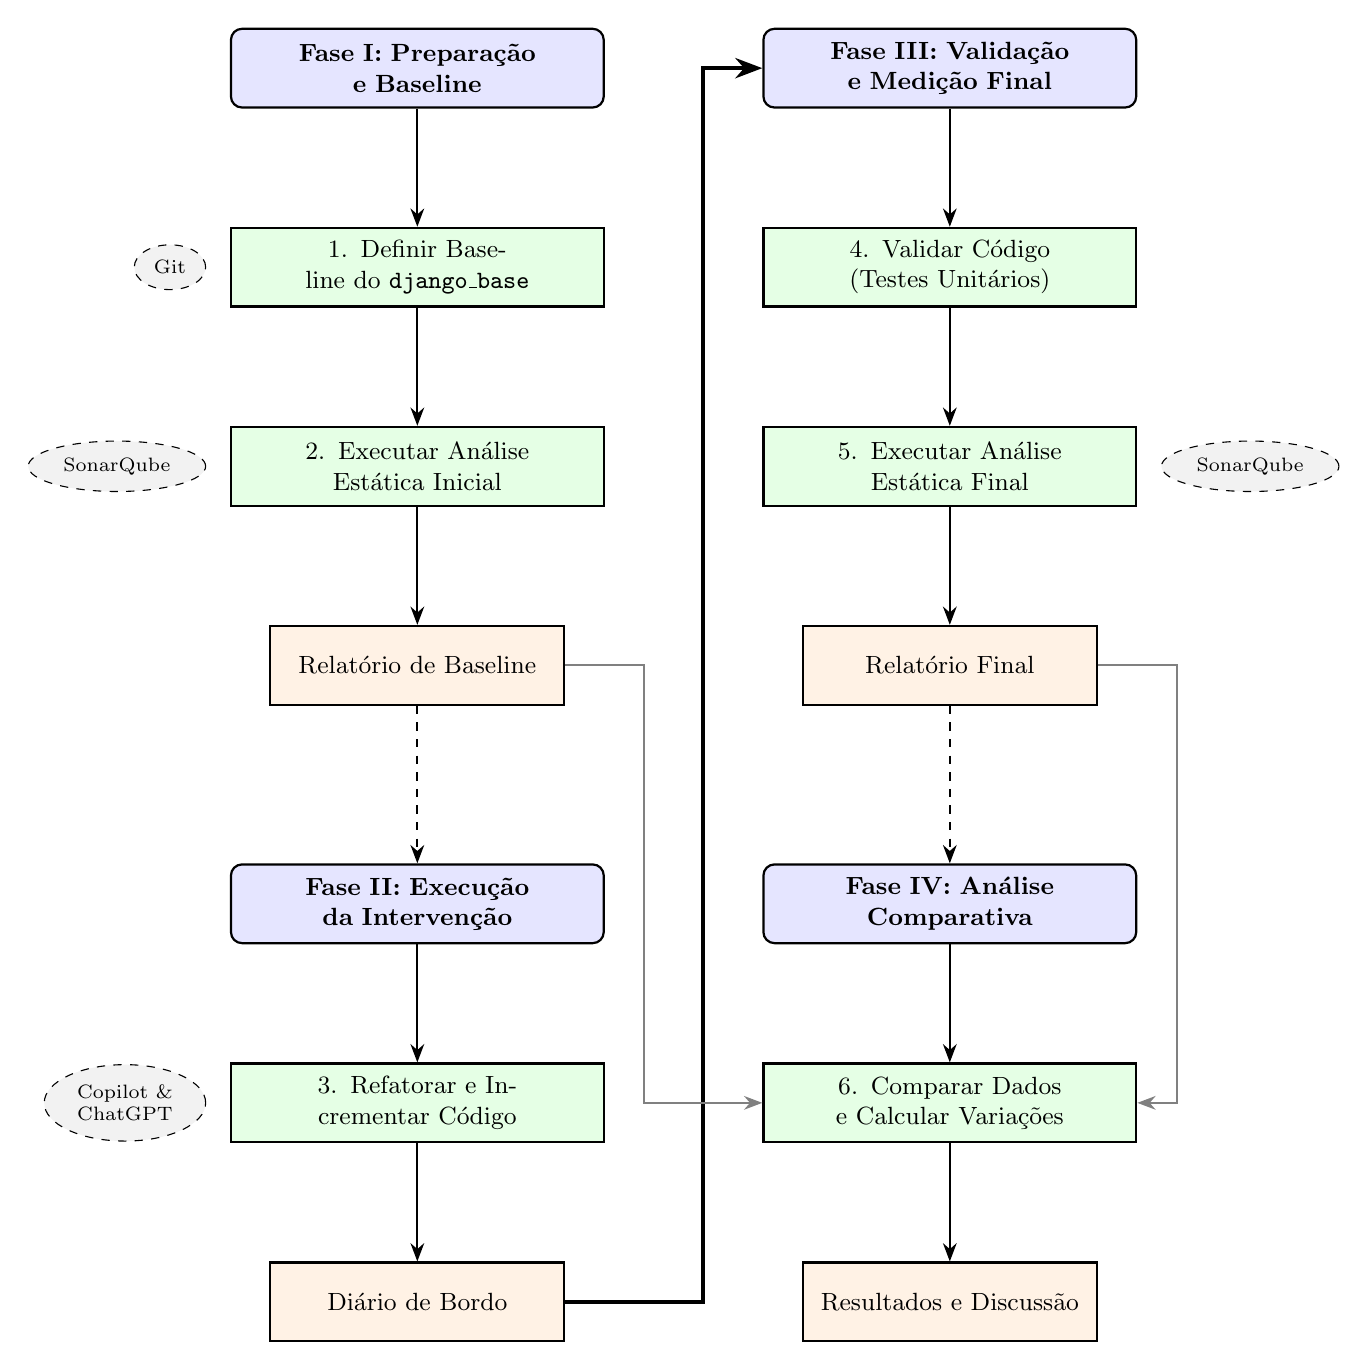
\begin{tikzpicture}[
        node distance=1.5cm and 2cm,
        font=\small,
        fase/.style={rectangle, rounded corners, draw, thick, fill=blue!10, text width=4.5cm, minimum height=1cm, align=center},
        processo/.style={rectangle, draw, thick, fill=green!10, text width=4.5cm, minimum height=1cm, align=center},
        artefato/.style={shape=rectangle, draw, thick, fill=orange!10, text width=3.5cm, align=center, minimum height=1cm},
        ferramenta/.style={shape=ellipse, draw, dashed, fill=gray!10, font=\scriptsize, align=center},
        conector/.style={-Stealth, thick}
    ]

    % FASE I
    \node[fase] (fase1) {\textbf{Fase I: Preparação e Baseline}};
    \node[processo, below=of fase1] (p1_isolar) {1. Definir Baseline do \texttt{django\_base}};
    \node[ferramenta, left=0.3cm of p1_isolar, anchor=east] (git1) {Git};
    \node[processo, below=of p1_isolar] (p2_analisar) {2. Executar Análise Estática Inicial};
    \node[ferramenta, left=0.3cm of p2_analisar, anchor=east] (sonar1) {SonarQube};
    \node[artefato, below=of p2_analisar] (a1_baseline) {Relatório de Baseline};
    
    % FASE II
    \node[fase, below=2cm of a1_baseline] (fase2) {\textbf{Fase II: Execução da Intervenção}};
    \node[processo, below=of fase2] (p3_desenvolver) {3. Refatorar e Incrementar Código};
    \node[ferramenta, left=0.3cm of p3_desenvolver, anchor=east] (ia) {Copilot \&\\ChatGPT};
    \node[artefato, below=of p3_desenvolver] (a2_diario) {Diário de Bordo};

    % --- COLUNA DA DIREITA (Fases III e IV) ---
    \node[fase, right=of fase1] (fase3) {\textbf{Fase III: Validação e Medição Final}};
    \node[processo, below=of fase3] (p4_validar) {4. Validar Código (Testes Unitários)};
    \node[processo, below=of p4_validar] (p5_analisar_final) {5. Executar Análise Estática Final};
    \node[ferramenta, right=0.3cm of p5_analisar_final, anchor=west] (sonar2) {SonarQube};
    \node[artefato, below=of p5_analisar_final] (a3_final) {Relatório Final};
    \node[fase, below=2cm of a3_final] (fase4) {\textbf{Fase IV: Análise Comparativa}};
    \node[processo, below=of fase4] (p6_comparar) {6. Comparar Dados e Calcular Variações};
    \node[artefato, below=of p6_comparar] (a4_resultados) {Resultados e Discussão};

    % --- CONECTORES ---
    \draw[conector] (fase1) -- (p1_isolar);
    \draw[conector] (p1_isolar) -- (p2_analisar);
    \draw[conector] (p2_analisar) -- (a1_baseline);
    \draw[conector] (fase2) -- (p3_desenvolver);
    \draw[conector] (p3_desenvolver) -- (a2_diario);
    \draw[conector] (fase3) -- (p4_validar);
    \draw[conector] (p4_validar) -- (p5_analisar_final);
    \draw[conector] (p5_analisar_final) -- (a3_final);
    \draw[conector] (fase4) -- (p6_comparar);
    \draw[conector] (p6_comparar) -- (a4_resultados);
    \draw[conector, dashed] (a1_baseline) -- (fase2);
    \draw[conector, dashed] (a3_final) -- (fase4);
    \draw[conector, line width=1.5pt] (a2_diario.east) -- ++(1.75,0) |- (fase3.west);
    \draw[conector, gray] (a1_baseline.east) -- ++(1,0) |- (p6_comparar.west);
    \draw[conector, gray] (a3_final.east) -- ++(1,0) |- (p6_comparar.east); 

    \end{tikzpicture}
    \caption{Fluxograma do desenho experimental pré e pós-intervenção, ilustrando o fluxo entre as fases de análise.}
    \label{fig:fluxograma_metodologia}
\end{figure}
% --- FIM DO CÓDIGO DO FLUXOGRAMA ---

\subsection{Evolução do Objeto de Estudo e Histórico}
Durante a fase inicial da pesquisa (TCC 1), o projeto \textit{open-source} \textbf{Zulip} foi selecionado como objeto de estudo para a aplicação das intervenções de IA. No entanto, durante a execução preliminar, identificou-se que a complexidade arquitetural do Zulip e, especificamente, a latência de seu pipeline de CI/CD (com tempos de execução de testes superiores a 30 minutos) inviabilizavam o ciclo rápido de \textit{feedback} necessário para medir a produtividade da IA em tempo real.

Além disso, a análise estática inicial do módulo selecionado no Zulip revelou uma cobertura de testes de apenas 22\%, o que criava uma linha de base ruidosa e dificultava a distinção entre o impacto da intervenção e a dívida técnica preexistente. Devido a esses impedimentos técnicos, o Zulip foi descontinuado como foco da intervenção ativa, sendo mantido neste trabalho apenas como registro das limitações metodológicas encontradas em projetos legados de alta complexidade.

\subsection{Seleção do Novo Objeto de Estudo: \texttt{django\_base}}
Para garantir a viabilidade e o rigor do experimento, o objeto de estudo foi substituído pelo projeto \textit{open-source} \textbf{\texttt{django\_base}} (v2.1.0), um template profissional para projetos Django desenvolvido pelos autores. Esta escolha foi fundamentada em:

\begin{itemize}
    \item \textbf{Linha de Base Robusta:} O projeto apresenta uma \textit{baseline} de alta maturidade (classificação "A" no SonarCloud e 93\% de cobertura de testes). Isso permite que ele sirva como um ambiente experimental controlado, onde o impacto da IA pode ser medido com precisão (sinal claro sem ruído).
    \item \textbf{Controle do Ambiente:} O domínio completo do ambiente elimina barreiras de infraestrutura, permitindo a execução rápida de ciclos de análise (Prompt $\rightarrow$ Código $\rightarrow$ Teste $\rightarrow$ Refatoração).
    \item \textbf{Arquitetura Modular:} A estrutura de Arquitetura Limpa do projeto é ideal para o desenho experimental de "evolução de software", permitindo que novos módulos sejam acoplados sem interferência no código legado.
\end{itemize}

Os resultados apresentados neste trabalho referem-se, portanto, exclusivamente às intervenções realizadas no \texttt{django\_base}.

\subsection{Ambiente e Ferramentas de Apoio}
Foi definido um ambiente de trabalho padronizado para garantir a consistência do experimento.
% ... (lista de ferramentas permanece idêntica) ...

\subsection{Definição do Escopo Experimental (Requisitos)}
\label{sec:requisitos_intervencao}
Para avaliar o impacto da IA em cenários de complexidade distintos, o experimento consiste em duas intervenções de desenvolvimento "greenfield" (código novo). A seguir, são especificados os requisitos para cada intervenção, que formarão o \textit{Product Backlog} do experimento.

\subsubsection{Intervenção A: Módulo de Lógica de Negócios (Carrinho de Compras)}
O objetivo é avaliar a capacidade da IA em lidar com lógica de negócios complexa e gerenciamento de estado.

\paragraph{Histórias de Usuário (Requisitos Funcionais)}
\begin{itemize}
    \item \textbf{HU-A1:} Como um usuário anônimo, eu quero adicionar um produto ao meu carrinho (baseado em sessão), para que eu possa comprá-lo mais tarde.
    \item \textbf{HU-A2:} Como um usuário anônimo, eu quero visualizar todos os itens e o valor total do meu carrinho, para que eu possa revisar meu pedido.
    \item \textbf{HU-A3:} Como um usuário anônimo, eu quero atualizar a quantidade de um item no meu carrinho, para que a lógica de cálculo do total seja re-executada.
    \item \textbf{HU-A4:} Como um usuário anônimo, eu quero remover um item do meu carrinho, para que eu não o compre.
\end{itemize}

\paragraph{Requisitos Não Funcionais}
\begin{itemize}
    \item \textbf{RNF-A1 (Testabilidade):} A lógica de negócios (cálculo de subtotal, total, adição e remoção) deve ser validada por testes unitários.
    \item \textbf{RNF-A2 (Manutenibilidade):} As funções e métodos do módulo devem manter uma Complexidade Ciclomática baixa (inferior a 10).
    \item \textbf{RNF-A3 (Confiabilidade):} A intervenção não deve introduzir nenhum `Bug` (classificação do SonarQube) no código novo.
\end{itemize}

\subsubsection{Intervenção B: Módulo de Segurança (Login Social OAuth2)}
O objetivo é avaliar a capacidade da IA em implementar um fluxo de segurança, uma área onde a literatura aponta riscos significativos.

\paragraph{Histórias de Usuário (Requisitos Funcionais)}
\begin{itemize}
    \item \textbf{HU-B1:} Como um novo usuário, eu quero me cadastrar/autenticar no sistema usando minha conta do Google, para não precisar criar uma conta local com senha.
    \item \textbf{HU-B2:} Como um usuário existente, eu quero fazer login usando minha conta do Google, para acessar minha conta rapidamente e de forma segura.
\end{itemize}

\paragraph{Requisitos Não Funcionais}
\begin{itemize}
    \item \textbf{RNF-B1 (Segurança):} O fluxo deve implementar o protocolo `Authorization Code Grant` do OAuth2.
    \item \textbf{RNF-B2 (Segurança):} As chaves secretas (API keys, client secrets) não devem estar expostas no código-fonte (\textit{hardcoded}), devendo ser lidas de variáveis de ambiente.
    \item \textbf{RNF-B3 (Segurança):} O código novo gerado não deve conter nenhuma `Vulnerabilidade` ou `Hotspot de Segurança` de criticidade alta ou média (classificação do SonarQube).
\end{itemize}

\subsubsection{Backlog do Produto Experimental}
A Tabela \ref{tab:backlog_experimento} consolida as \textit{features} (épicos) e suas respectivas histórias de usuário.

\begin{table}[htbp]
    \centering
    \caption{Backlog do Produto para o experimento de intervenção.}
    \label{tab:backlog_experimento}
    \begin{tabularx}{\textwidth}{l l X}
        \toprule
        \textbf{Feature (Épico)} & \textbf{ID da História} & \textbf{Descrição (História de Usuário)} \\
        \midrule
        \multirow{4}{*}{\parbox{3.5cm}{Gerenciamento de Carrinho de Compras}} 
        & HU-A1 & Adicionar produto ao carrinho (sessão). \\
        & HU-A2 & Visualizar carrinho e total. \\
        & HU-A3 & Atualizar quantidade de item no carrinho. \\
        & HU-A4 & Remover item do carrinho. \\
        \midrule
        \multirow{2}{*}{\parbox{3.5cm}{Autenticação via Google (OAuth2)}} 
        & HU-B1 & Cadastrar-se no sistema com conta Google. \\
        & HU-B2 & Fazer login no sistema com conta Google. \\
        \bottomrule
    \end{tabularx}
    \legend{Fonte: os Autores.}
\end{table}

\subsection{Arquitetura da Aplicação}
Foi definida e estruturada, com o auxílio do assistente de IA ChatGPT, a arquitetura final para a aplicação. O objetivo desse processo é entender como o agente de IA interpreta os requisitos e contribui para a definição arquitetural.

\subsubsection{Arquitetura sugerida pelo Agente}
A arquitetura para a intervenção no projeto \texttt{django\_base} foi desenhada para otimizar a testabilidade e a segurança. A estrutura segue o padrão nativo do Django, utilizando a separação por *Apps* de domínio e introduzindo uma \textbf{Camada de Serviço} para isolar a lógica de negócios.

\paragraph{Estrutura e Isolamento por Apps:}
O projeto será composto pelos seguintes Apps, garantindo o Princípio da Responsabilidade Única (SRP):
\begin{itemize}
    \item \texttt{shopping\_cart}: App responsável pela Intervenção A (Carrinho de Compras).
    \item \texttt{accounts}: App responsável pela Intervenção B (Segurança/OAuth2).
\end{itemize}

\paragraph{Camada de Serviço (Intervenção A):}
Para cumprir o RNF-A1 (Testabilidade) e RNF-A2 (Complexidade), toda a lógica complexa de gerenciamento é encapsulada em uma camada de serviço (\texttt{shopping\_cart/services.py}).
\begin{itemize}
    \item A \textbf{Camada de Serviço} manipula o estado do carrinho.
    \item As Views HTTP apenas delegam chamadas a esta camada e lidam com a resposta.
\end{itemize}

\paragraph{Segurança e Configuração (Intervenção B):}
Para atender aos requisitos de segurança (RNF-B1 a RNF-B3):
\begin{itemize}
    \item \textbf{Autenticação:} Utilização de bibliotecas consolidadas para implementar o fluxo \texttt{Authorization Code Grant}.
    \item \textbf{Segredos:} Todas as chaves devem ser lidas via \textbf{variáveis de ambiente} (\texttt{.env}), prevenindo a exposição no código-fonte.
\end{itemize}

\subsubsection{Desenho da Arquitetura Definida}
O desenho da arquitetura pode ser visualizado na Figura \ref{fig:diagrama_arquitetura}.

\begin{figure}[htbp]
    \centering
    \caption{Diagrama de Arquitetura de Software.}
    % Substitua pelo caminho correto da imagem da arquitetura
    \includegraphics[width=\textwidth]{figuras/TCC_Architecture_V1.png}
    \label{fig:diagrama_arquitetura}
    \legend{Fonte: os Autores.}
\end{figure}

O diagrama ilustra o isolamento dos domínios da intervenção (Carrinho e Segurança) e a separação de responsabilidades (SRP) dentro do projeto \texttt{django\_base}.

\paragraph{Níveis de Abstração e Componentes:}
\begin{enumerate}
    \item \textbf{Contêiner Principal (\texttt{django\_base}):} Representa o limite da aplicação.
    \item \textbf{Módulos Internos:}
    \begin{itemize}
        \item \textbf{Views/Interface:} Camada de entrada/saída que recebe requisições HTTP.
        \item \textbf{Lógica de Negócios (Serviços):} Contém as classes puras do \texttt{shopping\_cart/services.py}. É isolada e altamente testável.
        \item \textbf{Autenticação/Integração:} Lida com o fluxo de segurança do \texttt{accounts} App.
    \end{itemize}
    \item \textbf{Serviços Externos:} Componentes de infraestrutura necessários.
\end{enumerate}

\paragraph{Comunicações Críticas:}
\begin{itemize}
    \item \textbf{Fluxo Carrinho (Intervenção A):} A camada de Interface delega à Lógica de Negócios, que se comunica com o Sistema de Sessão.
    \item \textbf{Fluxo Segurança (Intervenção B):} A camada de Autenticação se comunica com o provedor OAuth2. A Configuração obtém chaves estritamente das Variáveis de Ambiente, cumprindo o RNF-B2.
\end{itemize}

\subsection{Definição das Métricas de Análise} \label{sec:metricas_analise}
% (Sem alteração nesta seção)
A seleção das métricas foi um processo deliberado...
% ... (Texto das métricas permanece idêntico) ...

\subsection{Critérios de Interpretação dos Resultados} \label{sec:interpretacao_resultados}
% (Sem alteração nesta seção)
% ... (Tabela de interpretação permanece idêntica) ...

\subsection{Protocolo de Execução do Experimento}
O protocolo experimental foi revisado para se adequar ao novo objeto de estudo. O processo será dividido em duas intervenções paralelas, executadas por pesquisadores distintos.

\subsubsection{Intervenção A: Módulo de Lógica de Negócios (Carrinho de Compras)}
\begin{itemize}
    \item \textbf{Pesquisador Responsável:} Lude Ribeiro.
    \item \textbf{Objetivo:} Implementar um novo módulo de "Carrinho de Compras" anônimo.
    \item \textbf{Hipótese a Validar:} Avaliar a capacidade da IA (Copilot e ChatGPT) em lidar com lógica de negócios complexa, gerenciamento de estado e geração de testes.
    \item \textbf{Indicadores-Chave:} Complexidade Ciclomática e Cobertura de Testes.
\end{itemize}

\subsubsection{Intervenção B: Módulo de Segurança (Login Social OAuth2)}
\begin{itemize}
    \item \textbf{Pesquisador Responsável:} Eric Chagas.
    \item \textbf{Objetivo:} Implementar a integração com um provedor de "Login Social" via OAuth2.
    \item \textbf{Hipótese a Validar:} Avaliar a eficácia da IA na implementação de fluxos de segurança, verificando a inserção de vulnerabilidades.
    \item \textbf{Indicadores-Chave:} Vulnerabilidades e Hotspots de Segurança (CodeQL/Sonar).
\end{itemize}

\subsubsection*{Fases de Execução (Aplicadas a cada Intervenção)}
Cada intervenção seguirá rigorosamente o mesmo protocolo de 4 fases em \textit{feature branches} Git separadas:

\subsubsection*{Fase I: Preparação}
\begin{enumerate}
    \item \textbf{Isolamento do Código-Fonte:} Criação de uma \textit{feature branch} a partir da \textit{main} (baseline).
    \item \textbf{Planejamento da Intervenção:} Definição dos requisitos específicos.
\end{enumerate}

\subsubsection*{Fase II: Execução da Intervenção (Desenvolvimento Assistido)}
\begin{enumerate}
    \setcounter{enumi}{2}
    \item \textbf{Desenvolvimento Assistido por IA:} Realização da codificação com o auxílio integral do GitHub Copilot e ChatGPT.
    \item \textbf{Registro Sistemático (Diário de Bordo):} Manutenção de um diário de bordo (disponível no Apêndice B) registrando os \textit{prompts}, sugestões acatadas/rejeitadas e justificativas.
\end{enumerate}

\subsubsection*{Fase III: Validação e Medição Final (Pós-Intervenção)}
\begin{enumerate}
    \setcounter{enumi}{4}
    \item \textbf{Validação Funcional:} Verificação de que o código compila e os testes passam.
    \item \textbf{Execução da Análise Estática:} Execução do SonarQube e `pytest-cov` na \textit{feature branch}.
    \item \textbf{Coleta de Dados Finais:} Arquivamento dos relatórios de qualidade.
\end{enumerate}

\subsubsection*{Fase IV: Análise Comparativa dos Resultados}
\begin{enumerate}
    \setcounter{enumi}{7}
    \item \textbf{Tabulação dos Dados:} Organização dos dados pós-intervenção.
    \item \textbf{Análise Crítica:} Avaliação da qualidade intrínseca do código gerado "do zero" pela IA, utilizando a \textit{baseline} de 93\% de cobertura como padrão-ouro.
    \item \textbf{Interpretação:} Análise dos resultados quantitativos, correlacionando-os com o Diário de Bordo.
\end{enumerate}

\subsection{Limitações da Metodologia}
\label{sec:limitacoes}
É imperativo reconhecer as limitações deste novo desenho de pesquisa.
\begin{itemize}
    \item \textbf{Generalização dos Resultados:} Por se tratar de um estudo de caso focado em um único projeto (\texttt{django\_base}), os resultados representam uma evidência pontual e aprofundada, não uma conclusão universal para todos os contextos de software.
    \item \textbf{Viés de Autoria e Familiaridade:} A principal limitação é o uso de um projeto de autoria de um dos pesquisadores. Isso introduz um viés de familiaridade que pode otimizar a interação com o código. No entanto, esta limitação é mitigada pela adoção de uma linha de base de alta maturidade (padrão rigoroso a ser mantido) e pelo uso de ferramentas de análise estática (SonarQube) como "árbitro" imparcial da qualidade.
\end{itemize}
    % \chapter[Resultados]{Resultados} \label{chapter:Resultados}

% O objetivo deste capítulo é realizar a exposição dos resultados obtidos por meio da realização deste trabalho, com ênfase nos objetivos alcançados. Os tópicos apresentados estão ordenados com base na execução das tarefas do projeto, sendo elas a \nameref{section:requisitosResultados}, o \nameref{section:gameDesignResultados}, o \nameref{section:desenvolvimentoResultados} e o \nameref{section:playtestingResultados}. As últimas seções, denominadas \nameref{section:Semex2024} e \nameref{section:Analise pos implementacao}, apresentam os resultados obtidos por meio da utilização do \textit{game} Math Hero em trabalhos realizados durante a semana de extensão da UnB no ano de 2024.

% \section{Elicitação de requisitos} \label{section:requisitosResultados}

% Na etapa de elicitação dos requisitos do projeto foi utilizada a técnica MoSCoW de priorização para definição da priorização de tarefas de desenvolvimento. Com base nos parâmetros da técnica, foram definidos, inicialmente, os requisitos descritos no Quadro \ref{quadro:Quadro de requisitos do Game Math Hero}.

% \begingroup
%     \begin{quadro} 
%     \caption{Requisitos iniciais do \textit{Game} Math Hero.}
%     \label{quadro:Quadro de requisitos do Game Math Hero}
%     \begin{center}
%         \begin{tabularx}{\linewidth}{|X|c|}
%             \hline
%             Requisito & Priorização \\
%             \hline
%             O \textit{game} Math Hero deve possuir código aberto & \textit{Must Have} \\
%             \rowcolor{Gray} O \textit{game} Math Hero deve facilitar a adição de plugins e personalizações & \textit{Should Have}\\
%             O \textit{game} Math Hero deve utilizar artes 2D & \textit{Must Have} \\
%             \rowcolor{Gray} O \textit{game Math Hero} deve possuir boa didática & \textit{Must Have}\\
%             O \textit{game} Math Hero deve utilizar linguagem acessível ao público alvo & \textit{Must Have} \\
%             \rowcolor{Gray} O \textit{game} Math Hero deve possuir um Modo história para aprendizado de técnicas de matemática mental & \textit{Must Have} \\
%             O \textit{game} Math Hero deve possuir um modo \textit{Time Attack} para competições entre jogadores & \textit{Must Have} \\
%             \rowcolor{Gray} O \textit{game} Math Hero deve ser multiplataforma (mobile e desktop) & \textit{Should Have} \\
%             O \textit{game} Math Hero não deve ter monetização associada & \textit{Must Have} \\
%             \rowcolor{Gray} O \textit{game} Math Hero deve possuir um modo tutorial para aprendizado das mecânicas do \textit{game} & \textit{Should Have} \\
%             O \textit{game} Math Hero deve ensinar técnicas de matemática mental & \textit{Must Have} \\
%             \hline
%         \end{tabularx}
%         \legend{Fonte: o Autor}
%     \end{center}
%     \end{quadro}
% \endgroup

% Como o processo de desenvolvimento de um jogo guiado pela engenharia de games é iterativo, ocorreram, ao longo do desenvolvimento do jogo, ocorreram, ao longo do desenvolvimento do jogo, mudanças nos requisitos descritos no Quadro \ref{quadro:Quadro de requisitos do Game Math Hero}. Foram removidos os requisitos referentes ao desenvolvimento do modo história do jogo, sendo eles: 
% \begin{itemize}
%     \item o \textit{game} Math Hero deve possuir boa didática; 
%     \item o \textit{game} Math Hero deve possuir um modo história para aprendizado de técnicas de matemática mental;
%     \item o \textit{game} Math Hero deve possuir um modo tutorial para aprendizado das mecânicas do game; e
%     \item o \textit{game} Math Hero deve ensinar técnicas de matemática mental.
% \end{itemize}

% Desde a versão inicial foi feita a transposição dos requisitos para tarefas que pudessem ser priorizadas e organizadas em um quadro de planejamento, além da criação do \textit{roadmap} do projeto, Estas tarefas e estes quadros foram atualizados e adaptados ao longo de todo o desenvolvimento, para refletir as decisões e adaptações necessárias.

% \section{Game Design} \label{section:gameDesignResultados}
% \begin{citacao}
% ``Frequentemente quando estivermos fazendo um game, começamos inserindo um objetivo ao qual o jogador deve alcançar. Mas, como levar o jogador do inicio do game até este objetivo, e mais importante, como fazer com que o jogador se divirta na jornada, é onde a parte complexa, mas divertida, começa'' \cite[min 1:10, tradução nossa]{brackeys_basic_2018}.\footnote{``\textit{Often when making a game, you start by setting a goal that the player has to acheive. But how to get the player from the beggining of the game and towards that goal, and most importantly, how to get the player to enjoy this journey, is where the tricky, and also fun part, comes into play}''}    
% \end{citacao}

% Na fase de \textit{game design} foi definido que o game Math Hero possuiria 2 modos jogáveis: um modo história, onde o jogador percorre um mundo fictício repleto de atividades relacionadas à matemática, onde por meio do aprendizado e aplicação de técnicas de matemática mental, o jogador poderia melhorar suas habilidades matemáticas e se divertir ao mesmo tempo; e um modo \textit{time attack}, que seria principalmente para competições, contendo métricas de números de erros e tempo gasto, mas também tem o intuito de estimular que os jogadores utilizem habilidades de matemática mental para solucionar questões matemáticas relacionadas às quatro operações básicas: adição, subtração, divisão e multiplicação.

% \subsection{Modo história}
%  Para o modo história do game foi definido como objetivo final do jogador: participar de um duelo matemático com um cientista maluco (Figura \ref{fig:cientista maluco}) para que ele pare com a loucura das expressões ``proibidas''. Para isso, o jogador deveria percorrer o laboratório do Professor R para retirar dali todos os seguidores do cientista maluco e recuperar o laboratório do professor, que está cheio de expressões matemáticas proibidas escritas em seus quadros (como divisões por zero, por exemplo).

% \begin{figure}[h]
%     \centering
%     \caption{Versão inicial do vilão do game \textit{Math Hero}}
%     \includegraphics[width=120pt, keepaspectratio]{figuras/cientista_maluco.pdf}
%     \label{fig:cientista maluco}
%     \legend{Fonte: o Autor}
% \end{figure}

% Por meio da conversa com os robôs (Figura \ref{fig:robos}) de ajuda do Professor R, o jogador aprenderia técnicas de matemática mental úteis no dia a dia, e também valiosas para superar os obstáculos (como portas travadas, enigmas nos quadros, itens trancados com senha, e mais) deixados pelos seguidores do cientista maluco nas salas do laboratório do Professor R.

% \begin{figure}[h]
%     \centering
%     \caption{Versão inicial dos robôs de ajuda do game \textit{Math Hero}}
%     \includegraphics[width=120pt, keepaspectratio]{figuras/robos.pdf}
%     \label{fig:robos}
%     \legend{Fonte: o Autor}
% \end{figure}

% Depois de definir o objetivo final e a jornada do jogador, foi preciso definir o estilo de arte, para que o game fosse atrativo para crianças e adolescente do ensino básico brasileiro. O estilo de arte escolhido foi o \textit{pixel art}, que traz facilidade de assimilação por parte dos jogadores por proporcionar simplicidade visual ao usuário final, além de facilitar a criação e animação dos \textit{assets} do game. O peronsagem principal (Figura \ref{fig:personagem principal}) do game é um(a) jovem aprendiz do Professor R.


% \begin{figure}[h]
%     \centering
%     \caption{Versão inicial do personagem principal do game \textit{Math Hero}}
%     \includegraphics[width=120pt, keepaspectratio]{figuras/personagem_principal.pdf}
%     \label{fig:personagem principal}
%     \legend{Fonte: o Autor}
% \end{figure}

% Na fase de level design do protótipo do game \textit{Math Hero}, a primeira etapa foi a criação e busca de \textit{assets} provisórios para desenvolver rapidamente as mecânicas propostas pela fase de elicitação de requisitos e de game design. O primeiro passo desta etapa foi a criação do \textit{sprite} do personagem principal do jogo utilizando o software Aseprite\footnote{\hyperlink{https://www.aseprite.org/}{https://www.aseprite.org/}}. Em seguida, foi necessário realizar a busca de um \textit{tilemap} provisório que atendesse às necessidades levantadas nos requisitos. Buscando por palavras chave como “2D, \textit{Science}, \textit{Lab} e \textit{Robots}”, foi possível encontrar um \textit{tilemap} que supriu as necessidades momentâneas do \textit{game} (Figura \ref{fig:tilemap-provisorio}).

% \begin{figure}[h]
%     \centering
%     \caption{Tilemap provisório}
%     \includegraphics[width=240pt, keepaspectratio]{figuras/tilemap-provisorio.pdf}
%     \label{fig:tilemap-provisorio}
%     \legend{Fonte: o Autor}
% \end{figure}

% % TODO
% A implementação do modo história avançou até a criação da fase tutorial, o que viabilizou a realização de duas sessões de \textit{playtesting} e a coleta de sugestões e opiniões relativas ao rumo a ser seguido no desenvolvimento deste modo. A continuação da implementação desse modo foi postergada para focar na implementação do modo de treino do \textit{time attack}, dada a oportunidade de aplicar o jogo durante a Semana de Extensão 2024 da UnB no evento ``Torneio de Matemática Mental 2024'' descrito na seção \nameref{section:Semex2024}.

% Com isso, na versão \textit{competition version}, o modo história está desabilitado e seus \textit{assets} foram removidos do projeto temporariamente, tendo em vista a diminuição do tamanho do arquivo executável do jogo, permitindo assim que o \textit{game} fosse instalado em máquinas com poucos recursos. Em trabalhos futuros envolvendo o Math Hero, o modo história deverá ser implementado levando em consideração os requisitos iniciais do projeto, para que o propósito do \textit{game} seja mantido.

% \subsection{Modo \textit{Time Attack}}
% No modo \textit{Time Attack} foi definido que existiriam 3 modos diferentes de jogo: normal, treinamento e competição. O modo normal contaria com todas as funcionalidades existentes no modo de jogo \textit{time attack}, porém não seria customizável e geraria cerca de 15 operações randômicas para o jogador. Já o modo treinamento possuiria a opção de selecionar quais operações ele deseja praticar e a \textit{seed} geradora das questões. Vale ressaltar também que nos modos citados acima o cronômetro seria desligado e os resultados não seriam salvos nem localmente nem em banco de dados próprio do \textit{game}.

% O modo competição, que é o alvo principal de estudo deste trabalho, seria customizável e rastreável, contendo as seguintes opções: seleção de tipos de operações, inserção de \textit{seed} geradora de questões aleatórias e armazenamento de resultados em um arquivo local ao computador. Foi planejado para um trabalho futuro o armazenamento em banco de dados em nuvem, para fácil acesso e coleta dos dados, tendo em vista que a coleta de dados é dificultada pelo deslocamento até o computador no qual o \textit{game} foi jogado.

% Em relação aos \textit{assets} utilizados no \textit{game design} do modo \textit{time attack}, foram obtidas inspirações imagens de telas de computadores antigos, e imagens de games que utilizam \textit{pixel art} como: Celeste\footnote{\hyperlink{https://www.celestegame.com/}{https://www.celestegame.com/}}, Shovel Knight\footnote{\hyperlink{https://www.yachtclubgames.com/games/shovel-knight-treasure-trove/}{https://www.yachtclubgames.com/games/shovel-knight-treasure-trove/}} e Fez\footnote{\hyperlink{https://store.steampowered.com/app/224760/FEZ/}{https://store.steampowered.com/app/224760/FEZ/}}.

% % TODO
% Dentre as três modalidades de \textit{time attack} inicialmente planejadas (modo competição, modo normal e modo treino), apenas uma mescla entre o modo treino e o modo competição foi implementada até o momento. O modo treino compartilha com o modo competição apenas a inserção de uma \textit{seed} para padronização dos resultados e a coleta dos dados após a finalização da resolução da sequência de expressões. As características não compartilhadas com o modo competição são: a ausência de penalidades para erros, a configuração livre de operações e não coletar os dados de jogo.

% Para a separação completa entre os dois modos de jogo, seria necessária a detecção do parâmetro de modo de jogo para que, ao selecionar o modo treino, as penalidades sejam desabilitadas, a configuração livre de operações seja possível e a coleta dos dados de jogo seja desabilitada. Já quando o parâmetro de modo de competição for selecionado, todas essas opções devem ser habilitadas, com exceção da livre configuração de operações, tendo em vista que a configuração de operações seria feita automaticamente, de acordo com a \textit{seed} da competição, facilitando assim a configuração do ambiente de competição e garantindo um ambiente justo e igual para todos os competidores.

% \section{Implementação} \label{section:desenvolvimentoResultados}

% A escolha da utilização da língua inglesa para o nome do jogo teve como motivação principal a intenção do lançamento do \textit{game} em plataformas digitais como o Itch.io e a Steam, facilitando a disseminação do jogo mundialmente.

% A primeira etapa da implementação foi a criação dos \textit{scripts} do \textit{game} utilizando a linguagem de \textit{scripting} própria da \textit{game} \textit{engine} escolhida, a \textit{GDScript}. Anteriormente, foi realizado estudo de boas práticas atreladas à linguagem e à Godot por meio de vídeos educativos propostos pela comunidade e pela documentação oficial da Godot.

% Em seguida, a próxima etapa realizada foi relacionada à implementação das mecânicas. Utilizando as boas práticas e a documentação da Godot \cite{godot_docs}, foi possível realizar a criação de \textit{scripts} específicos para a implementação de padrões arquiteturais de código, como o \textit{singleton} \textit{GameManager}, pode ser visualizado no Apêndice \ref{apendice: script GameManager}. %cada um dos modelos do game: personagem controlável (jogador), inimigo, NPC amigável e por fim, uma máquina de estados que tratará cada modelo que possuir mais de um estado que necessita de fluxos de controle próprios e de personalização de ações como movimentação (controlada pelo jogador ou via software), conversa, interações e etc. Os \textit{scripts} de controle do personagem, máquina de estados e o \textit{template} de estado podem ser encontrados nos Apêndices \ref{apendice: script character}, \ref{apendice: script state machine} e \ref{apendice: state template}, respectivamente.%

% %Remover scripts relacionados ao desenvolvimento do modo historia e adicionar scripts relevantes para o modo treino% 

% A estrutura de organização de arquivos definida para o projeto é apresentada pela Figura \ref{fig:estrutura-pastas}.
% A pasta \texttt{docs} contém toda a documentação do game gerada à partir da ferramenta \texttt{docsify}. A pasta \texttt{media} contém 4 subdivisões relacionadas à arquivos de mídia do jogo, sendo elas: \texttt{art}, que está relacionada aos \texttt{assets} de arte criados para o \textit{game}; \texttt{fonts}, que contém todos os arquivos de fontes necessários para as interfaces de usuário; \texttt{music}, que contém trilhas sonoras, música ambiente; e \texttt{sfx}: que contém todos os arquivos relativos aos efeitos sonoros. 

% \begin{figure}[h]
%     \centering
%     \caption{Estrutura de pastas Math Hero}
%     \includegraphics[width=240pt, keepaspectratio]{figuras/Estrutura de arquivos Math Hero.pdf}
%     \label{fig:estrutura-pastas}
%     \legend{Fonte: o Autor}
% \end{figure}

% A pasta \texttt{scenes} contém os arquivos com extensão \texttt{*.tscn} relativos às \textit{scenes} das diferentes fases do \textit{game}. Por último, a pasta \texttt{scripts} é a pasta que contém todos os \textit{scripts} escritos em \textit{GDScript}.

% Para a versão \textit{alpha} do \textit{game} o modo \textit{time attack} e seu modo de competição foram alvo do planejamento da implementação. Porém, a implementação real consistiu em fazer a produção de um mínimo produto viável (MVP) específico para os eventos descritos na seção \nameref{section:Semex2024}. O modo implementado, denominado modo de treino, possui uma versão inicial daquilo que foi planejado para o modo de competição contendo a inserção de \textit{seeds} para randomização e padronização das expressões a serem resolvidas pelo jogador, o registro de dados pertinentes ao modo de competição como: tempo decorrido, operações habilitadas e nome identificador; e a seleção da dificuldade de resolução das expressões. 

% A priorização do modo de treino deu-se pela emergente oportunidade de aplicação e validação do modelo e temática do jogo por meio de atividades como a \textit{SEMEX 2024} da UnB, onde foi proposto e planejado que o \textit{game} fosse utilizado para promover uma pequena competição matemática entre os participantes inscritos.

% \subsection{\textit{Time Attack}}

% Para desenvolver o modo \textit{time attack} do \textit{game}, primeiro fez-se necessário mapear os tipos de expressões para então definir as propriedades a serem utilizadas pelo jogador ao jogar este modo. As operações definidas, bem como suas propriedades, foram a adição, a subtração, a multiplicação e a divisão. As características referentes a cada operação e suas propriedades estão descritas nas Tabelas \ref{ops:add}, \ref{ops:sub}, \ref{ops:mul} e \ref{ops:div} respectivamente.

% % TODO
% Em todas as tabelas, foram consideradas apenas operações que geram resultados inteiros e positivos, isto é, com resultado $x \in \mathbb{Z}$ e $x \geq 0$.
% Na Tabela \ref{ops:add} estão separados os tipos de expressões de adição definidas para o modo \textit{time attack}. Levando em consideração expressões do tipo: $a+b=x$, a coluna ``Número de dígitos das parcelas'' representa o número de dígitos de cada parcela \textit{a} e \textit{b} e a coluna ``Vai um'' representa a utilização, ou não, da propriedade de ``vai um'' que ocorre quando a soma dos dígitos de centena, dezena ou unidade é maior ou igual a 10.

% \begin{table}[htbp]
% \begin{center}
%     \caption{Expressões disponíveis para a operação de adição}
%     \label{ops:add}
%     %\begin{tabular}{|c|c|}
%     \begin{tabular}{c|c}
%     \hline
%     \textbf{Número de dígitos das parcelas} & \textbf{``vai um''} \\
%     \hline
%         1 & \textcolor{red}{\faTimes} \\
%         \hline
%         1 & \textcolor{green!60!black}{\faCheck} \\
%         \hline
%         2 & \textcolor{red}{\faTimes} \\
%         \hline
%         2 & \textcolor{green!60!black}{\faCheck} \\
%         \hline
%         3 & \textcolor{red}{\faTimes} \\
%         \hline
%         3 & \textcolor{green!60!black}{\faCheck} \\
%     \hline
%     \end{tabular}
%     \legend{Fonte: o Autor}
% \end{center}
% \end{table}

% Já na Tabela \ref{ops:sub} estão dispostos os tipos escolhidos de expressões de subtração com base no modelo $a-b=x$. As colunas ``Dígitos de $a$'' e ``Dígitos de $b$'' representam a quantidade de dígitos de cada parcela \textit{a} e \textit{b} do modelo. A coluna ``Propriedade'' representa a propriedade utilizada nas parcelas \textit{a} e \textit{b} da expressão, um ``-'' representa que nenhuma propriedade especial foi utilizada. Por fim, a coluna ``Pegar emprestado'' representa a utilização, ou não, da propriedade de ``pegar emprestado'' ao solucionar a expressão. Essa propriedade ocorre quando a subtração de um dos dígitos de centena, dezena ou unidade representaria um resultado negativo, assim fazendo-se necessário ``pegar emprestado'' do dígito subsequente.

% \begin{table}[htbp]
% \begin{center}
%     \caption{Expressões $a - b$ disponíveis para a operação de subtração}
%     \label{ops:sub}
%     \begin{tabular}{c|c|c|c}
%     \hline
%     \textbf{Dígitos de $a$} & \textbf{Propriedade} & \textbf{Dígitos de $b$} &  \textbf{``pegar emprestado''} \\
%     \hline
%         1 & - & 1 & \textcolor{red}{\faTimes} \\
%         \hline
%         2 & Múltiplo de 10 & 1 & \textcolor{green!60!black}{\faCheck} \\
%         \hline
%         2 & - & 1 & \textcolor{red}{\faTimes} \\
%         \hline
%         2 & - & 1 & \textcolor{green!60!black}{\faCheck} \\
%         \hline
%         3 & Múltiplo de 100 & 2 & \textcolor{green!60!black}{\faCheck} \\
%         \hline
%         3 & - & 2 & \textcolor{red}{\faTimes} \\
%         \hline
%         4 & Múltiplo de 1000 & 3 & \textcolor{green!60!black}{\faCheck} \\
%         \hline
%         3 & - & 2 & \textcolor{green!60!black}{\faCheck} \\
%     \hline
%     \end{tabular}
%     \legend{Fonte: o Autor}
% \end{center}
% \end{table}

% Na Tabela \ref{ops:mul} foram expostos os tipos de expressões de multiplicação escolhidos para a implementação. Usando o modelo $a \times b = x$, as colunas ``Dígitos de $a$'' e ``Dígitos de $b$'' representam a quantidade de dígitos em cada uma das parcelas \textit{a} e \textit{b} da expressão. A coluna ``Propriedade'' apresenta as propriedades especiais utilizadas na expressão, e um ``-'' informa que nenhuma propriedade especial foi utilizada. Na coluna ``Vai um'', está representado a utilização, ou não, da propriedade de ``vai um'' na solução.

% \begin{table}[htbp]
% \begin{center}
%     \caption{Expressões $a \times b$ disponíveis para a operação de multiplicação}
%     \label{ops:mul}
%     \begin{tabular}{c|c|c|c}
%     \hline
%     \textbf{Dígitos de $a$} & \textbf{Propriedade} & \textbf{Dígitos de $b$} &  \textbf{``Vai um''} \\
%     \hline
%         1 & - & 1 & \textcolor{red}{\faTimes} \\
%         \hline
%         2 & $a = 11$ & 1 & \textcolor{green!60!black}{\faCheck} \\
%         \hline
%         2 & $a = 11$ & 2 & \textcolor{red}{\faTimes} \\
%         \hline
%         2 & $a = 11$ & 2 & \textcolor{green!60!black}{\faCheck} \\
%         \hline
%         2 & com 5 na unidade & 2 & \textcolor{green!60!black}{\faCheck} \\
%         \hline
%         2 & com 5 na dezena & 2 & \textcolor{green!60!black}{\faCheck} \\
%         \hline
%         3 & - & 2 & \textcolor{green!60!black}{\faCheck} \\
%         \hline
%         2 & $a = 11$ & 3 & \textcolor{red}{\faTimes} \\
%         \hline
%         2 & $a = 11$ & 3 & \textcolor{green!60!black}{\faCheck} \\
%         \hline
%         2 & - & 2 & \textcolor{green!60!black}{\faCheck} \\
%         \hline
%         3 & - & 3 & \textcolor{green!60!black}{\faCheck} \\
%     \hline
%     \end{tabular}
%     \legend{Fonte: o Autor}
% \end{center}
% \end{table}

% Por último, na Tabela \ref{ops:div} estão expostas as propriedades e o número de dígito de cada parcela de expressões do tipo: $a \div b = x$. onde a coluna ``Propriedade'' representa a utilização ou não de propriedades especiais na expressão.

% \begin{table}[htbp]
% \begin{center}
%     \caption{Expressões $a \div b$ disponíveis para a operação de divisão}
%     \label{ops:div}
%     \begin{tabular}{c|c|c}
%     \hline
%     \textbf{Dígitos de $a$} & \textbf{Propriedade} & \textbf{Dígitos de $b$}  \\
%     \hline
%         2 & - & 1 \\
%         \hline
%         2 & - & 2 \\
%         \hline
%         3 & - & 2 \\
%         \hline
%         2 & $b = 5$ & 1 \\
%         \hline
%         3 & - & 1 \\
%     \hline
%     \end{tabular}
%     \legend{Fonte: o Autor}
% \end{center}
% \end{table}

% \subsubsection{Escolha das referências}
% Conforme desenvolvimento do modo de jogo \textit{Time Attack}, foram utilizadas referências ``retrô'' para a criação dos \textit{assets} necessários para a criação da tela. Uma das principais referências foi a de telas de computador monocromáticas verdes, como pode ser observado na Figura \ref{fig:green pc screen}.

% \begin{figure}[h]
%     \centering
%     \caption{Tela de PC monocromática verde}
%     \includegraphics[height=240pt, keepaspectratio]{figuras/green pc screen.pdf}
%     \label{fig:green pc screen}
%     \legend{Fonte: Google Imagens}
% \end{figure}

% Também foi necessário selecionar a paleta de cores correspondente e realizar a criação dos \textit{assets} no software de criação de \textit{sprites} \textit{Aseprite}. A paleta de cores (Figura \ref{fig:pallete gameflower green}) escolhida tem o nome de \textit{Gameflower green} e foi obtida do site \href{https://lospec.com/}{lospec.com}.

% \begin{figure}[h]
%     \centering
%     \caption{Paleta de cores \textit{Gameflower green}}
%     \includegraphics[width=320pt, keepaspectratio]{figuras/pallete GameFlower Green.pdf}
%     \label{fig:pallete gameflower green}
%     \legend{Fonte: lospec.com}
% \end{figure}

% Com a utilização dessa paleta de cores, foi possível criar os \textit{assets} e renui-los no \textit{tileset} representado no Apêndice \hyperref[apendice: tilemap tattack]{\textit{Tilemap} do Modo \textit{Time Attack}}. Assim, unindo as referências buscadas à paleta de cores escolhida, a interface de batalha de matemática foi evoluída para a imagem apresentada na Figura \ref{fig:tela time attack}.

% \begin{figure}[h]
%     \centering
%     \caption{Tela do modo Time Attack}
%     \includegraphics[width=320pt, keepaspectratio]{figuras/Time attack screen.pdf}
%     \label{fig:tela time attack}
%     \legend{Fonte: o Autor}
% \end{figure}

% O primeiro protótipo da funcionalidade de batalha de matemática, que faria parte do modo história, pode ser visto na Figura \ref{fig:batalha matematica}. Conforme implementação do modo de treino, utilizado na \textit{SEMEX 2024} (Figura \ref{fig:versao competicao tattack}), o modo \textit{time attack} recebeu elementos gráficos que representam o tempo decorrido, a quantidade de erros, um teclado numérico para representação visual da seleção dos números, a \textit{seed} do jogo e as instruções visuais pertinentes ao modo, como o botão ``ENTER'' para confirmar o resultado da expressão e o botão ``ESC'' para pular a expressão atual e ir para a próxima, com uma penalidade de 30 segundos ao tempo final.%Conforme o progresso do desenvolvimento do game, a estilização, bem como novas regras foram adicionadas na batalha de matemática, para que a mesma interface seja utilizada tanto no modo quanto no modo \textit{Time Attack}. A utilização da mesma interface traz benefícios para a jogabilidade por proporcionar ao jogador uma interface simples e familiar em ambos os modos para que sua utilização e transição entre os diferentes modos de jogo seja a mais suave possível.

% \begin{figure}[h]
%     \centering
%     \caption{Evolução da mecânica utilizada no \textit{time attack}}
%     \begin{subfigure}[b]{0.45\linewidth}
%         \centering
%         \caption{Protótipo de mecânica de batalha}
%         \includegraphics[width=210pt, keepaspectratio]{figuras/batalha_matematica.pdf}
%         \label{fig:batalha matematica}
%         \legend{Fonte: o Autor}    
%     \end{subfigure}
%     \hfill
%     \begin{subfigure}[b]{0.45\linewidth}
%         \centering
%         \caption{\textit{time attack} versão competição}
%         \includegraphics[width=200pt, keepaspectratio]{figuras/Tela time attack.pdf}
%         \label{fig:versao competicao tattack}
%         \legend{Fonte: o Autor}    
%     \end{subfigure}
% \end{figure}

% \section{Playtesting} \label{section:playtestingResultados}

% A fase de \textit{playtesting} serviu como principal validadora da temática escolhida, mas também como medidor da aceitação da proposta do jogo. Nesta fase, foi importante aceitar todo tipo de \textit{feedbacks} e propostas de melhoria passadas pelos jogadores escolhidos para teste. Foram construídas duas personas fictícias, para preservação da identidade das pessoas, para realização do \textit{playtesting} e colheita de sugestões de melhorias, uma adolescente e uma adulta (Tabela \ref{table:personas playtesting 1}), e ambas jogaram a versão \textit{alpha} do jogo.

% \begingroup
%     \begin{table}[htbp]
%         \caption{Identificação das personas escolhidas para sessão de playtesting.}
%         \label{table:personas playtesting 1}
%     \begin{center}
%         \begin{tabular}{l c l}
%             \toprule
%             \textbf{Nome} & \textbf{Idade} & \textbf{\textit{Profissão}}\\
%             \midrule
%             Manuela & 15 & Estudante \\
%             \rowcolor{Gray} Pedro & 24 & Comunicador social\\
%             \hline
%         \end{tabular}
%         \legend{Fonte: o Autor}
%     \end{center}
%     \end{table}
% \endgroup

% \begin{figure}[h]
%     \centering
%     \caption{\textit{Scene} para realização de testes}
%     \includegraphics[width=330pt, keepaspectratio]{figuras/blocking math hero 1st level.pdf}
%     \label{fig:test level}
%     \legend{Fonte: o Autor}
% \end{figure}

% Durante a sessão de \textit{playtesting}, Manuela foi a principal fonte de coleta de dados e sugestões, visto que ela está dentro do público alvo e, portanto, traz uma visão do público alvo em relação ao produto final. A versão protótipo do game, representada pela Figura \ref{fig:test level}, possuia uma mecânica de movimentação limitada à fase em que o jogador se encontrava, além da mecânica de ``encontro'' com um NPC hostil, que chamava o jogador para uma batalha de matemática (Figura \ref{fig:batalha matematica}). As sugestões dadas por Manuela e Pedro após a sessão de \textit{playtesting}, e as observações feitas acerca do comportamento de ambos durante a sessão, estão descritas na Tabela \ref{table:feedbacks}.

% \begingroup
%     \begin{table}[htbp]
%         \caption{\textit{Feedbacks} dados pelas pessoas escolhidas para a sessão de \textit{playtesting}.}
%         \label{table:feedbacks}
%     \begin{center}
%         \begin{tabular}{l m{180pt} m{180pt}}
%             \toprule
%             \textbf{Nome} & \textbf{Sugestão} & \textbf{\textit{Observação}}\\
%             \midrule
%             Manuela & ``Achei muito entediante a batalha de matemática, seria legal se fosse tipo um \textit{escape room}, daí a pessoa precisaria de usar as técnicas pra encontrar pistas pra abrir as portas e passar de fase.''  & Jogadora iniciante mas teve facilidade na adequação aos controles. Sentiu falta de direcionamentos dados ao jogador \\
%             \rowcolor{Gray} Pedro & ``Achei boa a mecânica de batalha, mas bem lenta. Acho que poderia mudar ela e deixar tipo uma batalha com \textit{timer} rodando.'' & Jogador experiente. Sentiu falta de indicadores de progresso na fase.\\
%             \hline
%         \end{tabular}
%         \legend{Fonte: o Autor}
%     \end{center}
%     \end{table}
% \endgroup

% A principal sugestão foi fazer ajustes na jogabilidade para que o game se tornasse mais dinâmico, além de realizar ajustes na forma de progressão. A decisão tomada a partir dessa sugestão foi a de realizar um ajuste no game design para que o progresso se comportasse de forma similar à um ``\textit{escape room}'', onde os jogadores precisam encontrar pistas e solucionar problemas para progredir e, eventualmente, sair da sala onde se encontram atualmente para outra com novos desafios.

% Assim, foi possível planejar ajustes no \textit{game design}, para que o jogo seja mais atrativo para o usuário final e cumpra com o principal requisito de fortalecimento do aspecto lúdico do \textit{game}. Embora os ajustes e sugestões tenham sido levados em consideração na evolução da mecânica, elas não estão presentes no modo de treino, que foi desenvolvido como versão final deste trabalho, portanto a aplicação e coleta de novas sugestões e observações foram elencadas como tarefas para trabalhos futuros.

% \section{SEMEX 2024} \label{section:Semex2024}

% O \textit{game} Math Hero foi utilizado no evento ``Torneio de Matemática mental 2024'', entre os dias 04/11/2024 e 08/11/2024, no Campus UnB Gama: Faculdade de Ciências e Tecnologias em Engenharia. Foram ofertadas 60 vagas, onde 30 destas vagas foram destinadas ao turno matutino e as outras 30 ao turno vespertino. O evento foi guiado por um conjunto de regras básicas com a intenção de promover uma competição saudável e também como forma de padronizar a jogabilidade, fazendo com que os dados coletados fossem comparáveis
% As regras estabelecidas aos competidores em relação à execução do \textit{game} e ao comportamento de cada um dos competidores foram:

% \begin{enumerate}
%     \item O torneio de matemática mental é uma competição individual, onde os participantes se enfrentam, em turnos, para decidir quem consegue resolver problemas de adição, subtração, multiplicação e divisão mais rapidamente.
%     \item O programa utilizado pelos participantes é o Math Hero, software livre desenvolvido pelo estudante Matheus Pimentel Leal.
%     \item A cada rodada os participantes tentarão resolver 20 operações. As operações são as mesmas para todos os participantes: isto é garantido pela configuração prévia do modo competição. A organização do evento determinará qual será a configuração de cada rodada, e os participantes devem seguir as configurações à risca.
%     \item Caso o participante, por erro, descuido ou vontade própria, use uma configuração diferente da determinada pela organização, ele será eliminado da rodada, recebendo como tempo final 100 minutos.
%     \item Sendo uma competição individual, não é permitido, durante uma rodada, a comunicação com outros competidores ou o uso de calculadoras, celulares, internet, dispositivos eletrônicos ou papel e caneta. A violação desta regra implicará na desclassificação do competidor, que deverá deixar a competição.
%     \item A cada ciclo de duas rodadas serão classificados um certo número de competidores (a quantidade será divulgada pela organização a cada início de ciclo). Os não classificados deixam a competição.
%     \item A cada novo ciclo o nível de dificuldade das operações aumenta, partindo de iniciante até atingir o nível difícil.
%     \item A cada erro cometido o competidor adicionará uma penalidade de 30 segundos ao seu tempo final. Esta penalidade é computada automaticamente pelo Math Hero.
%     \item Caso o competidor deseje, ele pode saltar a operação atual, pagando uma penalidade de 5 minutos no seu tempo final.
%     \item O casos omissos serão tratados pela coordenação do evento.
% \end{enumerate}

% Em relação ao modelo da competição, foram definidas 3 etapas com 2 rodadas cada. Ao final da primeira rodada os 3 alunos com piores tempos foram eliminados e, ao final da segunda rodada, os 6 alunos com os piores tempos também foram eliminados. Dessa forma, na primeira rodada, pelo período da manhã, 31 alunos participaram da primeira rodada, 28 da segunda rodada e 22 da terceira rodada. E no período da tarde, 17 competidores participaram da primeira rodada, 14 da segunda rodada e, por último, 8 participaram da terceira rodada. 
% % 10 alunos foram eliminados a cada rodada. Assim, formando uma etapa final com 23 alunos, onde os 3 primeiros foram premiados com medalhas.

% O objetivo do evento ``Torneio de Matemática mental 2024'' era estimular a busca pelo conhecimento e desenvolvimento de técnicas facilitadoras para a realização de cálculos utilizando somente o fator mental, sem o auxílio de papéis, calculadoras ou quaisquer dispositivos que auxiliam na resolução de equações matemáticas.

%  Os alunos de uma escola de ensino médio do Gama foram convidados a participar do evento durante o período da manhã, como forma de incentivar e testar as habilidades dos mesmos em um ambiente lúdico. As técnicas de matemática mental apresentadas na Seção \nameref{section: matematica mental} do Capítulo \hyperref[chapter:Referencial Teórico]{Referencial Teórico} foram previamente ensinadas aos alunos com o auxílio de uma versão de testes do Math Hero. No total, 52 alunos participaram da competição. O resultado da competição na parte da manhã com os alunos de ensino médio pode ser observado por meio dos Tabela \ref{quadro: quadro de lideres manha}, que apresenta um ``top 10'' alunos ranqueados em ordem crescente pelo tempo total para resolução das expressões, no formato: $minutos:segundos:milissegundos$.
 
% \begin{table}[htbp]
% \centering
% \caption{Quadro de líderes de alunos de ensino básico treinados com as técnicas de matemática mental}
% \label{quadro: quadro de lideres manha}
% \rowcolors{2}{gray!15}{white}
% \begin{tabular}{l m{180pt} m{180pt}}
% \toprule
% \textbf{Posição} & \textbf{Nome}      & \textbf{Tempo Total} \\ \midrule
% 1  & Aluna A  & \texttt{005:03.564}            \\
% 2  & Aluna B  & \texttt{005:10.974}            \\
% 3  & Aluno C  & \texttt{005:35.395}            \\
% 4  & Aluna D  & \texttt{005:35.600}            \\
% 5  & Aluno E  & \texttt{007:12.161}            \\
% 6  & Aluno F  & \texttt{009:51.062}            \\
% 7  & Aluna G  & \texttt{010:18.884}            \\ 
% 8  & Aluno H  & \texttt{011:19.248}            \\ 
% 9  & Aluno I  & \texttt{011:59.204}            \\ 
% 10 & Aluna J  & \texttt{012:31.304}            \\  \bottomrule
% \end{tabular}
% \legend{Fonte: o Autor}
% \end{table}

% Como parâmetro de comparação, na parte da tarde a competição foi aberta ao público geral universitário, sem treinamento prévio de técnicas de matemática mental e sob as mesmas regras e estruturas utilizadas no período da manhã, para que fosse possível a análise do desempenho de pessoas sem instrução prévia sobre as técnicas de resolução mental. No período da tarde, no total compareceram 17 estudantes

% \begin{table}[htbp]
% \centering
% \caption{Quadro de líderes de alunos de ensino superior sem treinamento prévio com as técnicas de matemática mental}
% \rowcolors{2}{gray!15}{white}
% \begin{tabular}{l m{180pt} m{180pt}}
% \toprule
% \textbf{Posição} & \textbf{Nome}      & \textbf{Tempo Total} \\ \midrule
% 1  & Competidor A  & \texttt{005:15.583}            \\
% 2  & Competidor B  & \texttt{010:31.421}            \\
% 3  & Competidora C  & \texttt{010:55.652}            \\
% 4  & Competidor  D  & \texttt{011:04.054}            \\
% 5  & Competidora E  & \texttt{014:50.528}            \\
% 6  & Competidor F  & \texttt{015:28.875}            \\
% 7  & Competidor G  & \texttt{015:52.297}            \\ 
% 8  & Competidor H  & \texttt{070:00.000}            \\ \bottomrule
% \end{tabular}
% \legend{Fonte: o Autor}
% \end{table}

% Como podemos perceber, o desempenho dos alunos de ensino médio foi superior, considerando apenas o ``top 5'' de participantes no período da tarde e no período da manhã. O tempo médio para finalização das questões propostas dos ``\textit{top} 5'' participantes do período da manhã foi de: $5min 43s 539ms$. Já o tempo médio dos ``\textit{top} 5'' participantes do período da tarde foi de: $10min 31s 447ms$. Esta comparação sobre o desempenho de pessoas com e sem o conhecimento prévio reforça a validade da utilização de técnicas de matemática mental para a obtenção de resultados mais rápidos e corretos para expressões matemáticas. 

% % TODO
% O \textit{game} Math Hero teve um desempenho aceitável durante a realização do evento ``Torneio de matemática mental 2024''. Porém, algumas dificuldades foram encontradas, como a dificuldade de inserção das \textit{seeds} por parte de alguns alunos, fazendo com que alguns registros não fossem captados. Essa falha se deu por conta da funcionalidade de inserção manual das \textit{seeds}.

% Outro fato relevante foi a seleção de uma versão desatualizada do \textit{game} por parte de um estudante da turma de ensino médio, que foi o público do período da manhã. Esse fato se deu pela existência de uma versão do jogo instalada nos computadores do laboratório utilizado e de uma versão com atualizações de última hora que foi colocada na área de trabalho dos computadores do laboratório.

% De forma crítica, o resultado obtido pela utilização do jogo no evento foi satisfatório, mas com ressalvas. Melhorias nas funcionalidades do modo de treino e a criação do modo dedicado exclusivamente a competições foram as sugestões levantadas para realização de trabalhos futuros significativos para a evolução do software, além de proporcionar a realização de eventos com maior suavidade e menos dificuldades.

% % TODO
% \section{Análise pós-implementação} \label{section:Analise pos implementacao}
% % O texto ficou muito geral. Abra um pouco mais, em 4 ou 5 parágrafos, onde cada parágrafo foca em uma futura melhoria, falando o que ela seria, porque ela é importante, porque não foi implementada e como seria a implementação/relação dela com as já presentes e futuras
% A análise pós-implementação foi feita para que os pontos de dificuldade encontrados durante a utilização do \textit{game} Math Hero em competições de matemática mental tenham suas motivações encontradas e sanadas.

% % Separação dos modos treino e competição
% Na implementação atual do jogo, o modo implementado (modo \textit{time attack}) possui apenas uma modalidade, oriunda de uma mescla entre as modalidades de treino e de competição, utilizando características planejadas para ambos os modos. A separação completa entre as modalidades de competição e de treino inclui a adição de mais uma configuração de modo \textit{time attack}, que consiste em habilitar o cadastro prévio de \textit{seeds} de competição em um servidor remoto, para que, ao informar o código da competição como, por exemplo, ``\texttt{SEMEX2024}'', a \textit{seed} do jogo, juntamente com suas configurações de rodadas, sejam automaticamente carregadas, facilitando assim a configuração e utilização em eventos futuros. Esta funcionalidade não foi implementada devido a falta de organização prévia, dada urgência de utilização do \textit{game} no evento ``Torneio de matemática mental''. Com isso, optou-se por utilizar uma mescla entre as modalidades de treino e de competição levando em consideração a facilidade de implementação e a rapidez na entrega de um mínimo produto viável.

% % Adição de sistema de leaderboard de fácil acesso para competições
% Outra funcionalidade de suma importância para a utilização do \textit{software} em competições é a adição de um quadro de líderes que realize a exposição dos resultados, ordenados do menor tempo total até o maior tempo total. Este quadro de líderes teria facilitaria a organização e traria rapidez na divulgação dos resultados da rodada, bem como dos resultados finais.

% % Cadastro de seeds para competições
% Para melhorar consideravelmente a mão de obra necessária para realização de eventos, como o ``Torneio de matemática mental 2024'', é importante que seja implementado um cadastro de \textit{seeds} e de configurações de operações (habilitar ou não certas operações). Esse cadastro consiste em armazenar, remotamente, uma chave única para cada competição, bem como suas configurações, sendo elas: o número de rodadas, o tempo limite e as \textit{seeds} utilizadas em cada rodada.

% % Exportação do projeto para plataformas mobile
% Finalmente, para aumentar o alcance do jogo e fazer com que cada vez mais alunos do ensino básico e superior tenham acesso ao \textit{game}, será necessário exportar o jogo para plataformas como o Android e o iOS. Esta funcionalidade não foi implementada devido a falta de conhecimento prévio relacionado à publicação, aprovação e manutenção do software em lojas de aplicativos \textit{mobile}.
    \chapter{Cronograma de Execução e Gestão de Riscos}
\label{chap:cronograma}

Este capítulo apresenta o planejamento temporal e o registro da execução das atividades do TCC 2. Diferente de um cronograma linear tradicional, este plano de trabalho reflete a \textbf{natureza adaptativa} da pesquisa experimental. O cronograma foi reestruturado durante o curso do semestre para acomodar a decisão estratégica de substituição do objeto de estudo (Pivot), mitigando os riscos técnicos que ameaçavam a viabilidade do prazo final.

O cronograma final consolida-se em um regime de execução intensiva (\textit{Sprint}), visando a entrega do documento completo em \textbf{14 de Dezembro} e a defesa na data prevista de \textbf{16 de Dezembro}.

\section{Detalhamento das Fases e Adaptação do Plano}

A execução do projeto foi segmentada em quatro fases distintas. A Tabela \ref{tab:cronograma_tcc2_parte1} detalha a transição crítica da Fase 1 para a Fase 2, onde ocorreu a mudança de escopo técnico, e a Tabela \ref{tab:cronograma_tcc2_parte2} apresenta o planejamento final de escrita e defesa.

\begin{landscape}
    \begin{table}[htbp]
        \centering
        \caption{Cronograma Executivo TCC 2 - Fase Exploratória e Pivot (Ago/25 a Nov/25)}
        \label{tab:cronograma_tcc2_parte1}
        \begingroup
        \scriptsize
        % Ajustei as larguras para evitar Overfull \hbox
        \setlength{\tabcolsep}{4pt}
        \renewcommand{\arraystretch}{1.3}
        \begin{tabular}{@{} l p{8.5cm} c p{4.0cm} @{}}
            \toprule
            \textbf{Fase} & \textbf{Atividade e Descrição Detalhada} & \textbf{Período (Semanas)} & \textbf{Entregável / Marco} \\
            \midrule
            
            \multirow{3}{*}{\textbf{Fase 1}} & \textbf{Exploração e Baseline (Projeto Zulip):} Configuração de ambiente complexo, tentativa de isolamento de módulos e execução da análise estática inicial. Identificação de bloqueios de infraestrutura. & 18/08 a 31/10 (Sem. 1-10) & Relatório de Impedimentos Técnicos. \\
            \addlinespace[0.5em]
            & \textbf{Análise de Risco e Tomada de Decisão (Pivot):} Avaliação da inviabilidade do ciclo de feedback no Zulip. Seleção do \texttt{django\_base} como novo objeto de estudo. & 01/11 a 07/11 (Sem. 11) & \textbf{Marco de Decisão:} Troca de Objeto de Estudo. \\
            \addlinespace[0.5em]
            & \textbf{Setup do Novo Ambiente (django\_base):} Configuração do pipeline de CI/CD simplificado, Docker Compose e estabelecimento da nova Baseline de qualidade (SonarQube). & 08/11 a 17/11 (Sem. 12-13) & Nova Baseline ("Padrão Ouro") definida. \\
            \midrule
            
            \multirow{4}{*}{\textbf{Fase 2}} & \textbf{Intervenção Assistida por IA (Sprint de Desenvolvimento):} Implementação dos módulos de \textbf{Carrinho de Compras} (Lógica) e \textbf{Autenticação OAuth2} (Segurança) utilizando Copilot e ChatGPT. & \textbf{18/11 a 24/11 (Sem. 14)} & Código funcional, Testes e Diário de Bordo. \\
            \addlinespace[0.5em]
            & \textbf{Validação e Coleta de Métricas:} Execução de testes de regressão, testes de carga e nova análise estática (Pós-Intervenção). Coleta dos relatórios de cobertura. & 25/11 a 27/11 (Sem. 15) & Dados Brutos para Análise. \\
            \addlinespace[0.5em]
            & \textbf{Análise Quantitativa e Visualização:} Processamento dos dados, cálculo de delta (Antes vs. Depois) e geração dos gráficos comparativos. & 28/11 a 30/11 (Sem. 15) & Gráficos do Cap. de Resultados. \\
            \addlinespace[0.5em]
            & \textbf{Escrita do Capítulo de Resultados:} Redação técnica descrevendo os achados, correlacionando métricas com o Diário de Bordo. & 01/12 a 02/12 (Sem. 16) & Capítulo 4 Finalizado. \\
            \bottomrule
        \end{tabular}
        \endgroup
    \end{table}
\end{landscape}

\clearpage

\begin{landscape}
    \begin{table}[htbp]
        \centering
        \caption{Cronograma Executivo TCC 2 - Finalização e Defesa (Dezembro/25)}
        \label{tab:cronograma_tcc2_parte2}
        \begingroup
        \scriptsize
        \setlength{\tabcolsep}{4pt}
        \renewcommand{\arraystretch}{1.3}
        \begin{tabular}{@{} l p{8.5cm} c p{4.0cm} @{}}
            \toprule
            \textbf{Fase} & \textbf{Atividade e Descrição Detalhada} & \textbf{Período (Semanas)} & \textbf{Entregável / Marco} \\
            \midrule
            
            \multirow{3}{*}{\textbf{Fase 3}} & \textbf{Consolidação e Discussão:} Interpretação crítica dos resultados à luz do referencial teórico. Redação das Considerações Finais e Trabalhos Futuros. & 03/12 a 05/12 (Sem. 16) & Texto completo (Draft). \\
            \addlinespace[0.5em]
            & \textbf{Revisão Geral e Normalização ABNT:} Leitura completa, correção de citações, formatação de apêndices (Diário de Bordo e Protocolos) e revisão textual. & 06/12 a \textbf{13/12} (Sem. 17) & Versão Final para Depósito. \\
            \addlinespace[0.5em]
            & \textbf{Entrega Formal do Documento (DATA LIMITE):} Envio do documento final ao orientador e banca examinadora. & \textbf{14/12 (Sem. 17)} & \textbf{MARCO FINAL: ENTREGA.} \\
            \midrule
            
            \multirow{2}{*}{\textbf{Fase 4}} & \textbf{Preparação para Banca:} Elaboração dos slides, roteiro de apresentação e revisão dos principais pontos de arguição. & 10/12 a 15/12 (Sem. 17-18) & Material de Apresentação. \\
            \addlinespace[0.5em]
            & \textbf{Defesa Pública:} Apresentação do trabalho à banca examinadora. & \textbf{16/12 (Confirmado)} (Sem. 18) & \textbf{Conclusão do Curso.} \\
            \bottomrule
        \end{tabular}
        \endgroup
    \end{table}
\end{landscape}

\section{Visualização da Execução (Gantt)}
A Figura \ref{fig:gantt_cronograma} ilustra a distribuição temporal das atividades, destacando a extensão do prazo de escrita e revisão até a entrega final em 14/12.

\begin{figure}[htbp]
    \centering
    % Resizebox garante que o gráfico caiba na largura do texto sem estourar margem
    \resizebox{\textwidth}{!}{%
    \begin{ganttchart}[
        vgrid,
        hgrid,
        x unit=0.5cm,
        y unit chart=0.8cm,
        title height=1,
        bar/.style={fill=blue!50},
        bar incomplete/.style={fill=white},
        milestone/.style={fill=red!70},
        time slot format=simple
    ]{1}{18} 

    % --- CABEÇALHO ---
    \gantttitle{Cronograma TCC 2 - Execução e Pivot (2025)}{18} \\
    \gantttitle{Ago.}{2} 
    \gantttitle{Set.}{4}
    \gantttitle{Out.}{5}  
    \gantttitle{Nov.}{4}
    \gantttitle{Dez.}{3} \\
    \gantttitlelist{1,...,18}{1} \\

    % --- FASE 1: O PIVOT ---
    \ganttgroup[group/.append style={fill=gray!30}]{Fase 1: Exploração e Decisão}{1}{13} \\
    \ganttbar[bar/.append style={fill=gray!50}]{Tentativa Zulip (Impedimentos)}{1}{11} \\
    \ganttmilestone[milestone/.append style={fill=red!90}]{\textbf{Decisão de Pivot}}{11.5} \\
    \ganttbar{Setup Django Base}{12}{13} \\

    % --- FASE 2: EXECUÇÃO ---
    \ganttgroup[group/.append style={fill=blue!20}]{Fase 2: Intervenção (Sprint)}{14}{15} \\
    \ganttbar{\textbf{Dev. Assistido (Cart/Auth)}}{14}{14.5} \\
    \ganttbar{Validação e Métricas}{14.5}{15} \\ 
    \ganttbar{Análise de Dados}{15}{15.5} \\

    % --- FASE 3: ESCRITA E REVISÃO ---
    \ganttgroup[group/.append style={fill=green!30}]{Fase 3: Escrita Final}{16}{17} \\
    \ganttbar{Resultados e Discussão}{16}{16.5} \\
    \ganttbar{Revisão ABNT e Apêndices}{16.5}{17} \\
    \ganttmilestone[milestone/.append style={fill=orange!80}]
    {\textbf{ENTREGA (14/12)}}{17} \\

    % --- FASE 4: BANCA ---
    \ganttgroup[group/.append style={fill=yellow!30}]{Fase 4: Banca}{17}{18} \\
    \ganttbar{Prep. Apresentação}{17}{18} \\
    \ganttmilestone{\textbf{Defesa (16/12)}}{18}
    
    \end{ganttchart}
    }
    \caption{Linha do tempo do projeto, evidenciando o momento de decisão (Pivot) e o cronograma final até a defesa em 16/12.}
    \label{fig:gantt_cronograma}
\end{figure}
    % \chapter[Considerações finais]{Considerações Finais} \label{chapter:Conclusão e considerações finais}

Este trabalho propôs um jogo do gênero educacional chamado Math Hero, com o objetivo de introduzir técnicas de cálculo mental para alunos do ensino básico brasileiro por meio de uma abordagem lúdica, para que o estudante possa aprender de forma criativa e leve. Ao desenvolver um \textit{serious game} que não deixa o aspecto lúdico de lado, os jogadores poderão sentir-se em uma atividade recreativa ao mesmo tempo que aprendem por meio do aspecto educacional. 

Com a utilização das práticas recomendadas pela \textit{game software engineering} (GSE), o \textit{game} foi desenvolvido para ser relevante no meio pedagógico para o ensino de matemática. Os fatores de principal relevância foram a existência de modos de jogo que comportem tanto o ensino de técnicas de matemática mental quanto a utilização do jogo em competições que estimulem o aprendizado.

A dificuldade do balanceamento entre os aspectos lúdicos e educacionais foi notável durante o desenvolvimento do game. Percebeu-se que a introdução do aspecto educacional em um \textit{game} causa resistência por parte do público alvo por gerar sensação de obrigação relacionada ao desempenho. Por meio de sessões de \textit{playtesting} foi possível coletar \textit{feedbacks} para planejar ajustes no design do jogo para reduzir a sensação de obrigação e trazer divertimento aos jogadores durante o jogo no modo história. Os ajustes programados na realização de trabalhos futuros foram a exclusão da mecânica de batalha de matemática e a inclusão de obstáculos para fazer o \textit{game} ser como um ``\textit{escape room}''.

Outra dificuldade encontrada foi a escolha dos \textit{assets} do jogo. Esta escolha deve ser feita em concordância com os aspectos definidos no \textit{game design}, e por isso, muitas vezes os desenvolvedores optam por realizar a criação de \textit{assets} personalizados para cada game. Porém, com a restrição de tempo do projeto, não foi possível realizar a criação personalizada dos \textit{assets} para a solução visto a necessidade da validação do \textit{game design} proposto. Durante a procura de \textit{assets} personalizados, a barreira do preço de \textit{assets} disponibilizados no \textit{website icth.io} foi outra dificuldade que precisou ser superada.

A utilização da GSE foi um fator de sucesso no desenvolvimento do \textit{game} pois proporcionou a padronização de métodos e escolha de ferramentas adequadas para a solução. Tendo em vista o caráter iterativo da GSE, foi possível realizar validações e ajustes constantes no comportamento do jogo.

A escolha de ferramentas alinhadas com os requisitos definidos inicialmente trouxe facilidade de desenvolvimento por proporcionar padronização de configuração entre máquinas de trabalho com diferentes sistemas operacionais.

\section{Análise dos objetivos}
% Comentar que este objetivo não foi concluído: desenvolver um modo de jogo que cative o jogador por meio de elementos narrativos a aprender técnicas de matemática mental;
Considerando os objetivos específicos expostos na seção \nameref{section:Objetivos} da \hyperref[chapter:Introdução]{Introdução}, a implementação do jogo Math Hero satisfez os objetivos específicos: 
\begin{itemize}
    \item aplicar padrões de \textit{game design} atrativos para o público alvo;
    \item coletar, no mínimo, os seguintes dados de jogabilidade do modo competitivo: tempo decorrido até a finalização, nome do jogador, configuração das questões e \textit{seed} de jogo; e
    \item analisar os resultados obtidos a partir dos dados de jogabilidade dos jogadores.
\end{itemize}

Padrões de \textit{game design} foram aplicados por meio da utilização de referências modernas para construção dos \textit{assets} utilizados na implementação. Os dados de tempo decorrido até a finalização, nome do jogador, configuração das questões e da \textit{seed} do jogo foram coletados e armazenados localmente em um diretório específico do \textit{game}, criado automaticamente durante a finalização das questões e inserção do nome do jogador.

Já os resultados obtidos por meio de sessões de \textit{playtesting} foram analisados e levados em consideração para o planejamento e implementação de funcionalidades futuras e melhorias na execução e jogabilidade do Math Hero.

Por fim, os objetivos específicos não satisfeitos em sua totalidade foram:
\begin{itemize}
    \item desenvolver um modo de jogo que cative o jogador por meio de elementos narrativos a aprender técnicas de matemática mental; e
    \item adicionar um modo de jogo competitivo que estimule o aprendizado e a competição saudável.
\end{itemize}

O desenvolvimento de um modo de jogo que funcionasse como um ``modo história'' não foi realizado para ceder espaço para o desenvolvimento de um mínimo produto viável que atendesse as necessidades do evento ``Torneio de matemática mental'' realizado na Semana de Extensão Universitária 2024 da UnB, dada a grande oportunidade de coletar dados que suportem o ensino de técnicas de matemática mental no ensino básico. E, pelo mesmo motivo, a configuração de competição do modo \textit{time attack} não foi implementada em sua totalidade, dando espaço para uma mescla entre a configuração de treino e de competição.

% Por fim, as atividades planejadas (descritas na Tabela \ref{table:Atividades de desenvolvimento 2}), salvo as que ainda não puderam ser levantadas, estão alinhadas com o desenvolvimento e entrega de um game pronto e em concordância com os requisitos e necessidades do público alvo. O desenvolvimento e artes personalizadas, execução do processo iterativo descrito pela GSE e o design do game dão o escopo geral do planejamento de desenvolvimento do projeto.

\section{Trabalhos futuros}

Um dos mais importantes trabalhos futuros planejados é a continuidade do desenvolvimento do \textit{Math Hero}, além da liberação das próximas versões do \textit{game}, que contarão com o modo história completo e refatorado, um quadro de líderes para modo \textit{time attack}, além de novos modos, sendo estes um modo de treino e um modo normal sem a postagem do tempo no quadro de líderes. Também estão sendo planejadas versões do jogo para plataformas \textit{mobile} e \textit{web}, com o intuito de ampliar o alcance do \textit{game}.

A aplicação eficaz das sugestões levantadas até o momento possibilitará a evolução constante do projeto, bem como a sua utilização em diferentes contextos. Uma melhoria significativa seria a implementação completa do modo história do jogo, utilizando a temática de ``\textit{escape room}'' para validação e realização de novas sessões de coleta de \textit{feedbacks} através do \textit{playtesting}.

    \bookmarksetup{startatroot} 

    %\postextual

    \bibliography{bibliografia} 
    %\begin{anexosenv}

\chapter{Máquina de estados em \textit{GDScript}}
\begin{figure}[h]
    \caption{Máquina de estados em \textit{GDScript}}
    \begin{small}
    \begin{verbatim}
    extends Node
    class_name StateMachine

    @export var initial_state: State

    var current_state: State
    var states: Dictionary = {}

    func _ready():
	    for child in get_children():
		        if child is State:
			             states[child.name.to_lower()] = child
			             child.Transition.connect(on_child_transition)
		
		        if initial_state:
			             initial_state.Enter()
			             current_state = initial_state

    func _process(delta: float):
	       if current_state:
		          current_state.Update(delta)

    func _physics_process(delta: float):
	    if current_state:
		          current_state.Physics_Update(delta)

    func on_child_transition(state: State, new_state_name: String):
	    if state.name.to_lower() != current_state.name.to_lower():
		          return

	    var new_state = states.get(new_state_name.to_lower())
        if !new_state:
            return
	
        if current_state:
            current_state.Exit()

            new_state.Enter()
            current_state = new_state
    \end{verbatim}
    \end{small}
\end{figure}

\chapter{Template de um estado em \textit{GDScript}}
\begin{figure}[h]
    \caption{\textit{Template} de um estado em \textit{GDScript}}
    \begin{verbatim}
        extends Node
        class_name State
    
        signal Transition
    
        func Enter():
        	   pass
        func Exit():
        	   pass
        func Update(_delta: float):
        	   pass
        func Physics_Update(_delta: float):
        	   pass
    \end{verbatim}
\end{figure}

\end{anexosenv}


    \begin{apendicesenv}

% ===========================================================================
% APÊNDICE A: MAPEAMENTO ISO/IEC 25010 (Manutenibilidade)
% ===========================================================================
\chapter{Mapeamento das Métricas de Manutenibilidade}
\label{apendice:map_manut}

\begin{table}[H]
    \centering
    \scriptsize
    \caption{Relação entre as métricas de Manutenibilidade do estudo e as subcaracterísticas da norma ISO/IEC 25010:2023 \cite{isoiec25010}.}
    \label{tab:apendice_manutenibilidade}
    \begin{tabularx}{\textwidth}{l X X}
        \toprule
        \textbf{Subcaracterística} & \textbf{Métrica (SonarQube)} & \textbf{Relação e Alinhamento} \\
        \midrule
        \textbf{Analisabilidade} & \textbf{Dívida Técnica} & Medida em tempo de remediação, indica o esforço para entender e consertar o código. Alto nível de dívida compromete a analisabilidade. \\
        \cmidrule{2-3}
        & \textbf{Code Smells} & Tornam o código complexo de diagnosticar. A redução melhora a facilidade de análise. \\
        \midrule
        \textbf{Modificabilidade} & \textbf{Complexidade Ciclomática} & Funções complexas são difíceis de modificar. O controle garante modificações seguras. \\
        \cmidrule{2-3}
        & \textbf{Código Duplicado} & Exige mudanças em múltiplos locais, aumentando risco de erros. \\
        \midrule
        \textbf{Testabilidade} & (Cobertura de Testes) & Embora crítica, a cobertura complementa a análise de manutenibilidade. \\
        \bottomrule
    \end{tabularx}
\end{table}

% ===========================================================================
% APÊNDICE B: MAPEAMENTO ISO/IEC 25010 (Confiabilidade)
% ===========================================================================
\chapter{Mapeamento da Métrica de Confiabilidade}
\label{apendice:map_conf}

\begin{table}[H]
    \centering
    \scriptsize
    \caption{Relação entre a métrica de Confiabilidade do estudo e as subcaracterísticas da norma ISO/IEC 25010:2023 \cite{isoiec25010}.}
    \label{tab:apendice_confiabilidade}
    \begin{tabularx}{\textwidth}{l X X}
        \toprule
        \textbf{Subcaracterística} & \textbf{Métrica (SonarQube)} & \textbf{Relação e Alinhamento} \\
        \midrule
        \textbf{Tolerância a Falhas} & \textbf{Bugs} & Bugs são a manifestação direta de problemas de confiabilidade. Sua redução aumenta a confiança no sistema. \\
        \bottomrule
    \end{tabularx}
\end{table}

% ===========================================================================
% APÊNDICE C: MAPEAMENTO ISO/IEC 25010 (Segurança)
% ===========================================================================
\chapter{Mapeamento das Métricas de Segurança}
\label{apendice:map_seg}

\begin{table}[H]
    \centering
    \scriptsize
    \caption{Relação entre as métricas de Segurança do estudo e as subcaracterísticas da norma ISO/IEC 25010:2023 \cite{isoiec25010}.}
    \label{tab:apendice_seguranca}
    \begin{tabularx}{\textwidth}{l X X}
        \toprule
        \textbf{Subcaracterística} & \textbf{Métrica (SonarQube)} & \textbf{Relação e Alinhamento} \\
        \midrule
        \textbf{Integridade} & \textbf{Vulnerabilidades} & Correção de falhas que permitem exploração do sistema. \\
        \cmidrule{2-3}
        \textbf{Confidencialidade} & \textbf{Hotspots de Segurança} & Pontos sensíveis que exigem revisão manual para garantir proteção de dados. \\
        \bottomrule
    \end{tabularx}
\end{table}

% ===========================================================================
% APÊNDICE D: PROTOCOLO DE REPRODUCIBILIDADE
% ===========================================================================
\chapter{Protocolo de Reproducibilidade Experimental}
\label{apendice:protocolo_reproducibilidade}

Este apêndice documenta os artefatos de configuração utilizados. O objetivo é permitir a reprodução do experimento, contrastando a complexidade do projeto inicial (Zulip) com a solução otimizada (Django Base).

\section{Ambiente 1: Projeto Zulip (Fase Exploratória)}
A complexidade da infraestrutura de testes do Zulip inviabilizou o ciclo de feedback rápido. Abaixo, o trecho do arquivo \texttt{zulip-ci.yml} que demonstra a dependência de contêineres customizados e scripts proprietários.

\begin{verbatim}
jobs:
  tests:
    strategy:
      matrix:
        include:
          - docker_image: zulip/ci:jammy
            name: Ubuntu 22.04 (Python 3.10)
    container: ${{ matrix.docker_image }}
    steps:
      - name: Install dependencies
        run: |
          ./tools/ci/setup-backend --skip-dev-db-build
      - name: Run backend tests
        run: |
          ./tools/test-backend --coverage
\end{verbatim}

\section{Ambiente 2: Projeto Django Base (Ambiente Ativo)}
Ambiente onde as intervenções foram executadas. Utiliza padrões de mercado para garantir reprodutibilidade.

\subsection{Containerização (Docker Compose)}
Trecho do arquivo \texttt{docker-compose.dev.yml} utilizado:

\begin{verbatim}
services:
    project:
        container_name: project_dev
        build:
            context: .
            dockerfile: Dockerfile.dev
        ports:
            - "8000:8000"
        depends_on:
            project_db:
                condition: service_healthy

    project_db:
        image: postgres:13-alpine
        healthcheck:
            test: ["CMD-SHELL", "pg_isready -U postgres"]
            interval: 5s
\end{verbatim}

\subsection{Automação (Makefile)}
Comandos utilizados para padronizar a execução dos testes e análises.
\textit{Nota: Os emojis originais foram removidos para compatibilidade com a compilação do documento.}

\begin{verbatim}
# Execucao da suite de testes completa
test:
    @echo "[TEST] Executando testes..."
    @cd $(PROJECT_DIR) && . ../$(VENV)/bin/activate && \
    export PYTHONPATH=$$PWD && $(PYTEST) -v core cart

# Medicao de cobertura para o Sonar
test-coverage:
    @echo "[COVERAGE] Executando testes com cobertura..."
    @cd $(PROJECT_DIR) && . ../$(VENV)/bin/activate && \
    export PYTHONPATH=$$PWD && \
    $(PYTEST) --cov=core --cov=cart --cov-report=xml

# Analise de Seguranca
security-check:
    @echo "[SECURITY] Verificando vulnerabilidades..."
    @cd $(PROJECT_DIR) && . ../$(VENV)/bin/activate && pip-audit
\end{verbatim}

\subsection{Pipeline CI/CD (GitHub Actions)}
Configuração do \textit{workflow} para validação contínua.

\begin{verbatim}
name: CI/CD Pipeline
on: [push, pull_request]
jobs:
  test-and-quality:
    runs-on: ubuntu-latest
    steps:
      - name: Set up Python
        uses: actions/setup-python@v4
        with:
          python-version: "3.12"
      - name: Run tests
        run: |
          cd project
          pytest --cov=core --cov=cart --cov-report=xml:coverage.xml
      - name: SonarCloud Scan
        uses: SonarSource/sonarcloud-github-action@master
\end{verbatim}

% ===========================================================================
% APÊNDICE E: DIÁRIO DE BORDO (EXPANDIDO)
% ===========================================================================
\chapter{Diário de Bordo Experimental}
\label{apendice:diario_bordo}

Este apêndice apresenta o registro cronológico e detalhado das sessões de pareamento com as ferramentas de IA. O objetivo é documentar não apenas o código final, mas o processo de construção, incluindo as falhas de contexto, as alucinações da ferramenta e as intervenções humanas corretivas.

\section*{Entrada 1: Definição Arquitetural e Configuração Inicial}
\label{diario:entrada1}
\textbf{Data:} 24/11/2025

\begin{table}[H]
    \centering
    \small
    \begin{tabularx}{\textwidth}{|l|X|}
        \hline
        \textbf{Pesquisador} & Lude Ribeiro \\ \hline
        \textbf{Requisito} & Arquitetura do Módulo (Modular Monolith) \\ \hline
        \textbf{Ferramenta} & ChatGPT 4.0 (Web) \\ \hline
        \textbf{Tempo} & aproximadamente 4 horas \\ \hline
    \end{tabularx}
\end{table}

\textbf{1. Objetivo:} Definir a estrutura de pastas para o novo módulo \texttt{cart} respeitando a Clean Architecture já existente.

\textbf{2. Interação (Prompt):}
\begin{quote}
"Atue como um Arquiteto de Software. Preciso criar um NOVO módulo isolado chamado \texttt{cart}. Forneça um script bash para criar a árvore de diretórios e a configuração do \texttt{apps.py}."
\end{quote}

\textbf{3. Resultado e Análise:}
A IA gerou um script tecnicamente correto, mas posicionalmente errado. Ela assumiu a raiz do repositório git como raiz do projeto Django.
\begin{itemize}
    \item \textbf{Falha:} O script criaria pastas fora de \texttt{project/}.
    \item \textbf{Intervenção Humana:} Execução manual do script dentro do diretório correto.
    \item \textbf{Conclusão:} A IA carece de "consciência espacial" do projeto sem acesso direto à árvore de arquivos.
\end{itemize}

\section*{Entrada 2: A Crise de Infraestrutura e Perda de Contexto}
\label{diario:entrada2}
\textbf{Data:} 25/11/2025

\begin{table}[H]
    \centering
    \small
    \begin{tabularx}{\textwidth}{|l|X|}
        \hline
        \textbf{Requisito} & Configuração de Ambiente (Docker) \\ \hline
        \textbf{Ferramenta} & ChatGPT 4.0 (Web) \\ \hline
    \end{tabularx}
\end{table}

\textbf{1. Incidente:} Durante o setup, ocorreu um erro de rede no Docker (\texttt{IPv6 network unreachable}).
\textbf{2. Impacto no Experimento:} A sessão de debugging consumiu mais de 40 interações. Ao tentar retornar ao código Python, a IA sofreu \textbf{Saturação de Contexto}, "esquecendo" as definições arquiteturais feitas na Entrada 1 e sugerindo código fora do padrão estabelecido.

\section*{Entrada 3: Falha na Implementação da API e Pivô de Ferramenta}
\label{diario:entrada3}
\textbf{Data:} 26/11/2025

\begin{table}[H]
    \centering
    \small
    \begin{tabularx}{\textwidth}{|l|X|}
        \hline
        \textbf{Requisito} & Implementação de Views e Serializers \\ \hline
        \textbf{Ferramenta} & ChatGPT (Web) $\rightarrow$ \textbf{Migração para GitHub Copilot} \\ \hline
    \end{tabularx}
\end{table}

\textbf{1. Problema (Loop de Erro):}
Ao tentar implementar o \texttt{CartViewSet}, o ChatGPT gerou um código que resultava em \texttt{400 Bad Request}. Ao ser confrontado com o erro, a ferramenta entrou em contradição, sugerindo alterações cíclicas entre \texttt{ModelViewSet} e \texttt{GenericViewSet} sem resolver a causa raiz (validação do serializer).

\textbf{2. Decisão Metodológica (Pivot):}
Diagnosticou-se que a ferramenta baseada em chat era insuficiente para refatoração de múltiplos arquivos interdependentes. Optou-se pela migração para o \textbf{GitHub Copilot Agent} no VS Code, utilizando a flag \texttt{@workspace} para leitura de contexto local.

\section*{Entrada 4: Implementação de Lógica Complexa (Service)}
\label{diario:entrada4}
\textbf{Data:} 27/11/2025

\begin{table}[H]
    \centering
    \small
    \begin{tabularx}{\textwidth}{|l|X|}
        \hline
        \textbf{Ferramenta} & GitHub Copilot Agent \\ \hline
        \textbf{Requisito} & Regras de Negócio: Estoque e Atomicidade \\ \hline
    \end{tabularx}
\end{table}

\textbf{1. Prompt Técnico:}
\begin{quote}
"@workspace Implemente a lógica de \texttt{add\_item} no \texttt{CartService}. Requisitos: Validação de estoque (lançar ValueError), Snapshot de preço e garantia de atomicidade de banco de dados."
\end{quote}

\textbf{2. Resultado (Sucesso):}
A IA gerou uma implementação robusta:
\begin{itemize}
    \item Usou \texttt{transaction.atomic} e \texttt{select\_for\_update} corretamente para evitar \textit{Race Conditions}.
    \item Sugeriu proativamente a extração da validação para um método privado \texttt{\_validate\_stock}, reduzindo a complexidade ciclomática (Atendendo RNF-A2).
\end{itemize}

\section*{Entrada 5: Testes Automatizados e Correção de Configuração}
\label{diario:entrada5}
\textbf{Data:} 28/11/2025

\begin{table}[H]
    \centering
    \small
    \begin{tabularx}{\textwidth}{|l|X|}
        \hline
        \textbf{Requisito} & RNF-A1 (Cobertura de Testes) \\ \hline
        \textbf{Resultado} & \textbf{92\% de Cobertura} no Módulo Cart \\ \hline
    \end{tabularx}
\end{table}

\textbf{1. Incidente de Configuração:}
Ao rodar os testes gerados, ocorreu o erro \texttt{RuntimeError: Model class ... isn't in INSTALLED\_APPS}.
\textbf{2. Correção Assistida:}
O Copilot analisou o workspace e identificou que, embora o app estivesse no \texttt{settings.py} principal, ele estava ausente do \texttt{settings\_test.py} usado pelo Pytest. A IA gerou o patch de correção imediatamente.

\section*{Entrada 6: Refinamento de API (Correção de URLs)}
\label{diario:entrada6}
\textbf{Data:} 09/12/2025

\begin{table}[H]
    \centering
    \small
    \begin{tabularx}{\textwidth}{|l|X|}
        \hline
        \textbf{Requisito} & UX da API e Padrões REST \\ \hline
        \textbf{Problema} & Redundância nas rotas (\texttt{/cart/v1/cart/...}) \\ \hline
    \end{tabularx}
\end{table}

\textbf{1. Análise Humana:}
A inspeção do Swagger revelou URLs mal formadas devido à configuração padrão do \texttt{DefaultRouter} do DRF sugerida pela IA.

\textbf{2. Ação Corretiva:}
Solicitou-se a correção do \texttt{urls.py} para registrar a rota base como vazia, normalizando os endpoints para \texttt{/cart/v1/add\_item/}. Isso exigiu a atualização subsequente de todos os testes de integração que quebraram (Regressão).

\section*{Entrada 7: Refinamento Semântico (Remoção de Paginação)}
\label{diario:entrada7}
\textbf{Data:} 10/12/2025

\begin{table}[H]
    \centering
    \small
    \begin{tabularx}{\textwidth}{|l|X|}
        \hline
        \textbf{Requisito} & Semântica de Negócio (Carrinho Único) \\ \hline
        \textbf{Problema} & Endpoint GET retornava lista paginada \\ \hline
    \end{tabularx}
\end{table}

\textbf{1. Problema Semântico:}
A IA aplicou o padrão genérico de "Listagem" do Django Rest Framework, retornando uma estrutura paginada (`count`, `results: [...]`) para o endpoint de visualização do carrinho.
\textbf{2. Intervenção Humana:}
O pesquisador identificou que, semanticamente, um usuário possui apenas \textbf{um} carrinho ativo. Foi solicitado à IA que sobrescrevesse o método \texttt{list} do ViewSet para retornar o objeto direto, simplificando o consumo pelo frontend.

\textbf{3. Conclusão da Intervenção A:}
Com este ajuste final, o módulo atingiu os critérios de qualidade funcional, semântica e de cobertura, encerrando-se a fase de desenvolvimento do Carrinho.

\end{apendicesenv}
    %\printindex

\end{document}

